%!TEX root = ../terrainbook.tex
% chktex-file 46


\setchapterpreamble[u]{\margintoc}
\labch{acquisition}

\graphicspath{{acquisition/}}


\chapter{Acquisition of elevation measurements}%
\label{chap:acquisition}

The very first step in the process of terrain modelling is the acquisition of elevation measurements. 
Nowadays, these measurements are usually collected in large quantities using some form of remote sensing, \ie\ sensors that measure---in our case---the distance to the Earth's surface from an airborne or even a spaceborne platform. 
In raw form, elevation measurements are typically stored as a point cloud, \ie\ a collection of georeferenced 3D points with each point representing one elevation measurement on the Earth's surface.

There are a number of remote sensing techniques that are used to measure elevation on Earth or other planets. 
Typically, these techniques measure 1) the distance to the target surface and 2) their own position and orientation with respect to some global reference system. 
By combining these, we can compute the 3D coordinates of the measured location on the target surface. 

In this chapter we will focus primarily on lidar, the most common acquisition technique for large scale terrain models with centimetre level accuracy. 
But we also give an overview of other acquisition techniques, for example photogrammetry, InSAR, and sonar. 
And to conclude we will look at typical artefacts that you might encounter while working with elevation data. 
This is because, as with any kind of real-world measurements, there are various uncertainties and restrictions in the acquisition process that lead to distortions---the \emph{artefacts}---in the acquired data. These artefacts need to be taken into account when further processing and using the elevation data. 
%This often makes further processing of the data more difficult, because these artefacts often violate assumption that are made in the DTM algorithms used to further process and analyse the point cloud, leading to erroneous results. 
% It is important that you are aware of these artefacts while working with elevation data, because only then you will be able to make the right modelling decisions. 
%Section~\ref{sec:artefacts} gives an overview of common problems in elevation data.

\section{Principles of lidar}%
\label{sec:lidar-principles}

A lidar system\footnote{While `lidar' is often treated as the acronym of \textbf{li}ght \textbf{d}etection \textbf{a}nd \textbf{r}anging, it actually originated as a portmanteau of `light' and `radar'. Source \url{https://en.wikipedia.org/wiki/Lidar\#History\_and\_etymology}} measures the distance to a target by illuminating it with pulsed laser light and measuring the reflected or \emph{backscattered}\footnote{Backscattering is the natural phenomenon of  the reflection of (electromagnetic) waves or signals back to the direction they came from.} signal with a sensor (see Figure~\ref{fig:acqLidar}). 
\marginnote{time-of-flight}\index{time-of-flight}
\index{acqLidar}
\begin{marginfigure}
	\centering
	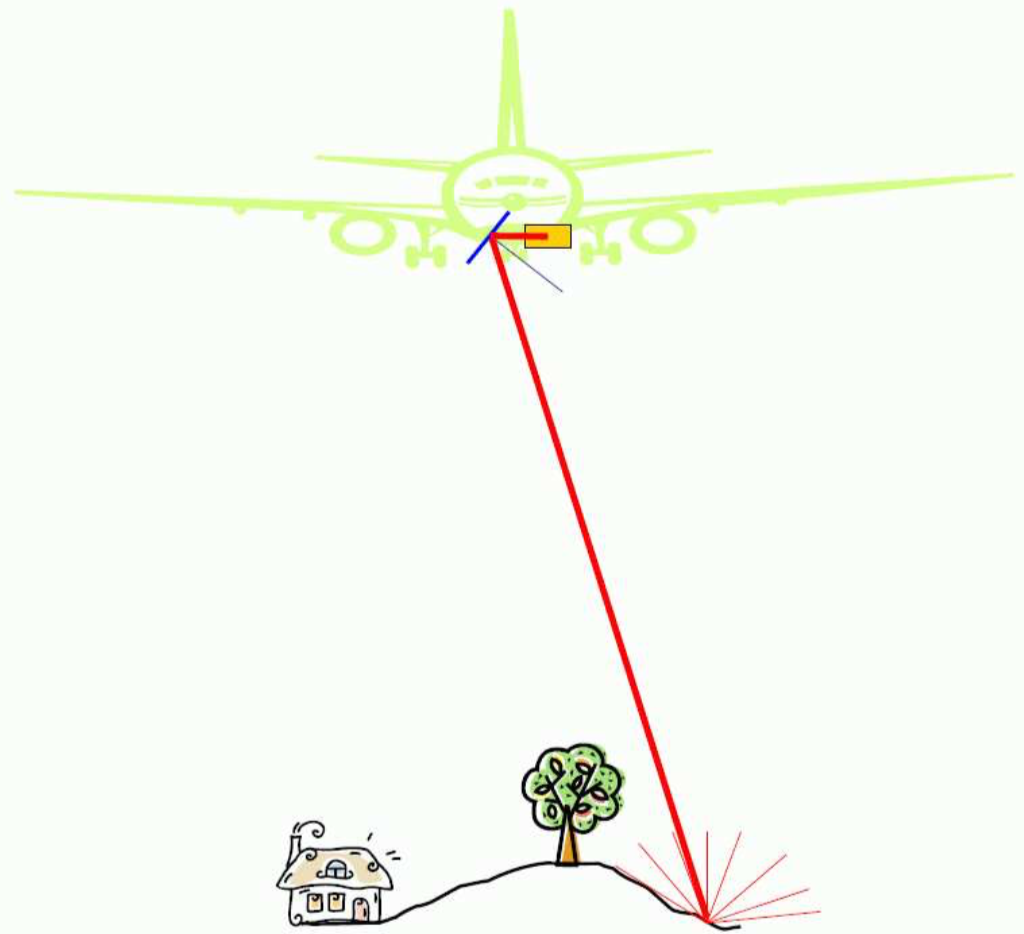
\includegraphics[width=\textwidth]{figs/lidar.png}
	\caption{Lidar range measurment}%
	\label{fig:acqLidar}
\end{marginfigure}
By measuring the time-of-flight, \ie\ the difference in time between emitting a pulse and detecting its return or \emph{echo}, the distance to the target that reflected the pulse can be found using a simple formula. To be exact, the time-of-flight $T$ is equal to
\begin{equation}
	\label{eq:tof}
	T= 2 \frac{R}{c}
\end{equation}
where $c$ is the speed of  light (approximately 300,000 km/s), and $R$ is the distance or \emph{range} between the lidar scanner and the target object that reflects the laser pulse. Therefore the range $R$ can be found from the measured time-of-flight $T$ using
\begin{equation*}
	R = \frac{1}{2} Tc.
\end{equation*}
A typical lidar systems performs hundreds of thousands of such range measurements per second. 

Lidar scanners exist in various forms. 
They can be mounted on a static tripod (terrestrial lidar) for detailed local scans, or on a moving platform such as a car (mobile lidar) or an aircraft (airborne lidar) for rapid scanning of larger areas. Nowadays, also hand-held lidar systems exist, and even some of the latest smartphones  have a lidar sensor. Furthermore, lidar can also be used from a satellite in space\footnote{NASA has used space lidar on earth (\url{https://en.wikipedia.org/wiki/ICESat-2}), on the Moon (\url{https://lola.gsfc.nasa.gov}), and on Mars (\url{https://en.wikipedia.org/wiki/Mars_Orbiter_Laser_Altimeter}).}. 

However, in the remainder of this text we will focus on airborne lidar.


%%%
%
\subsection{Georeferencing the range measurements}

\begin{figure}
	\centering
	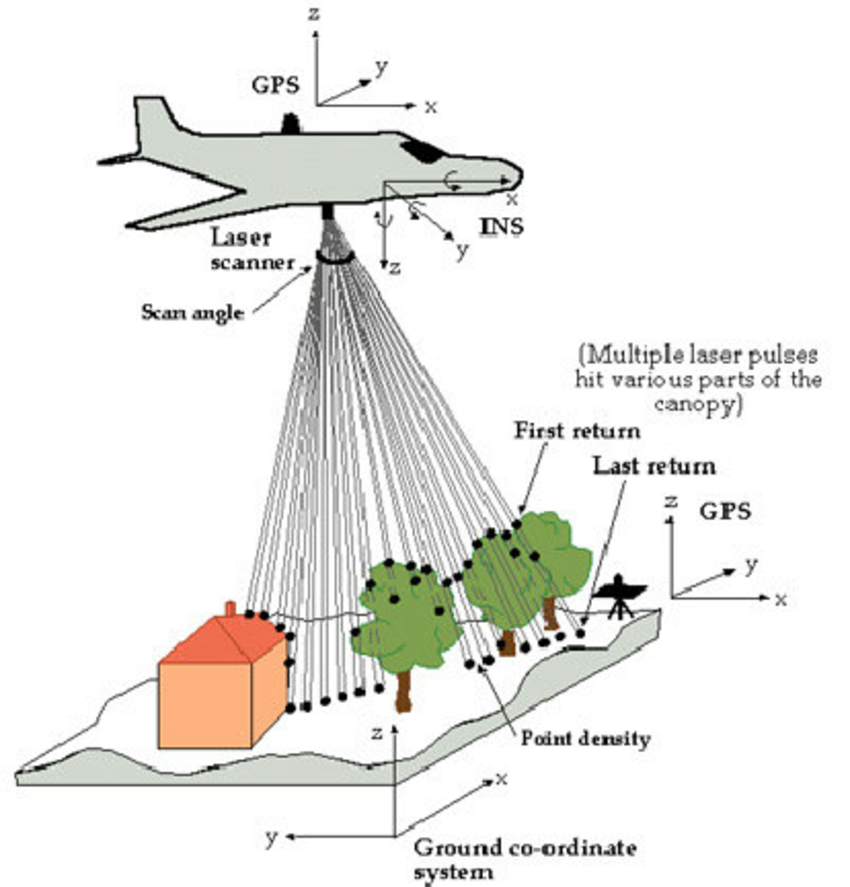
\includegraphics[width=0.7\textwidth]{figs/lidar-gnss-imu.png}
	\caption{An airborne lidar system. Figure from \citet{Dowman04}.}%
\label{fig:airborne-lidar}
\end{figure}
Apart from the  laser scanner itself, a lidar  system uses a GPS receiver and an inertial navigation system (INS), see Figure~\ref{fig:airborne-lidar}. 
\marginnote{inertial navigation system (INS)}\index{inertial navigation system (INS)}
These devices, which respectively provide the global position and orientation of the laser scanner, are needed for georeferencing, \ie\ to convert the range measurements of the laser scanner to 3D point measurements in a global coordinate system such as WGS84. 

To  obtain an accurate global position, \emph{differential GPS} (DGPS) is employed. 
\marginnote{differential GPS}\index{differential GPS}
DGPS is a technique to enhance the accuracy of GPS  by using GPS stations on the ground (one is visible in Figure~\ref{fig:airborne-lidar}). 
These DGPS stations have a known position and they broadcast the difference between that  known position and the position at the station as indicated by GPS\@. 
This difference is essentially a correction for errors in the GPS signal. The aircraft receives these differences from nearby DGPS stations and uses them to correct the GPS position of the aircraft. Using DGPS the accuracy of the GPS position on the aircraft can be improved from around 15 meters to several centimetres.

To obtain the accurate orientation of the laser scanner, the INS of the aircraft is used. 
The INS accurately measures the orientation, \ie\ the yaw, pitch  and roll angles of the aircraft, by means of an inertial measurement unit (IMU)\footnote{\url{https://en.wikipedia.org/wiki/Inertial_measurement_unit}}. 
\marginnote{inertial measurement unit (IMU)}\index{inertial measurement unit (IMU)}
Only when we accurately know the orientation of the laser scanner, can we know the direction (in a global coordinate system) in which a laser pulse is emitted from the aircraft.

By combining the global position and the global orientation of the laser scanner with the range measurement from the laser scanner, the georeferenced 3D position of  the point  on the target object that reflected the lase pulse can be computed.


%%%
\subsection{Echo detection}

A lidar system performs ranging measurements using the time-of-flight principle that allows us to compute range from a time measurement using the known speed of light in the air. 
The time measurement starts when the laser pulse is emitted and is completed when a backscattered echo of that signal is detected. 
In practice one emitted pulse can even lead to multiple echoes  in the case when an object reflects part of the laser pulse, but also allows part of the pulse to continue past the object. 
Notice that lidar pulses are typically emitted in a slightly divergent manner. As a result the footprint of the pules at ground level is several centimetres in diameter, which increases the likelihood of multiple echoes.

\begin{figure}
	\centering
	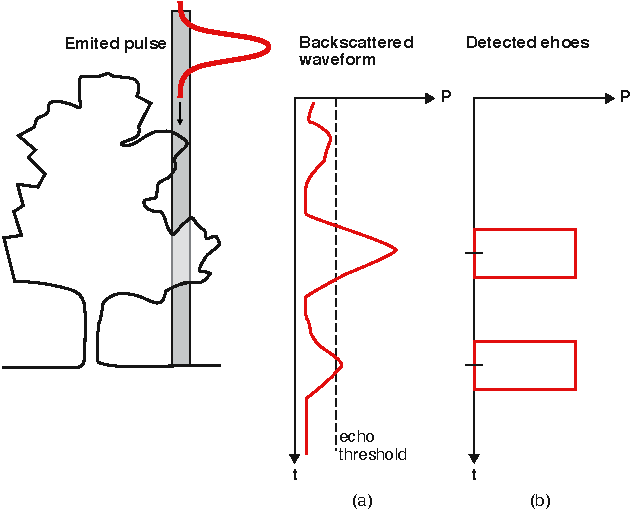
\includegraphics[width=0.8\textwidth]{figs/lidar-multipulse.pdf}
	\caption{The emitted laser pulse, \textbf{(a)} the returned signal, and \textbf{(b)} the recorded echoes. Figure adapted from \citet{Bailly12}.}%
\label{fig:lidar-multipulse}
\end{figure}
Figure~\ref{fig:lidar-multipulse} illustrates what the backscattered signal looks like when it hits a target object in the shape of a tree. 
A tree is particularly interesting because it often causes multiple echoes (one or more on its branches and one on the ground below).  The lidar sensor observes a waveform that represents the received signal power ($P$) as a function of time ($t$). 
With the direct detection lidar systems that we focus on in this book, the echoes are derived from the backscattered waveform by using a thresholding technique. This essentially means that an echo is recorded whenever the power of the waveform exceeds a fixed threshold (see Figure~\ref{fig:lidar-multipulse}b). 

An echo can  also  be referred to as a \emph{return}. 
\marginnote{return}\index{return}
For each return the return count is recorded, \eg\ the first return is the first echo received from an emitted laser pules and the last return is the last received echo (see Figure~\ref{fig:lidar-multipulse}). The return count can in some cases be used to determine if an echo was reflected on vegetation or ground (ground should then be the last return).


%%%
\subsection{Anatomy of a lidar system}%
\label{lidar:anatomy}

A lidar system consists of an optical and an electronic part. 
As shown in Figure~\ref{fig:lidar-components}, each part consists of several components.
\begin{figure}
	\centering
	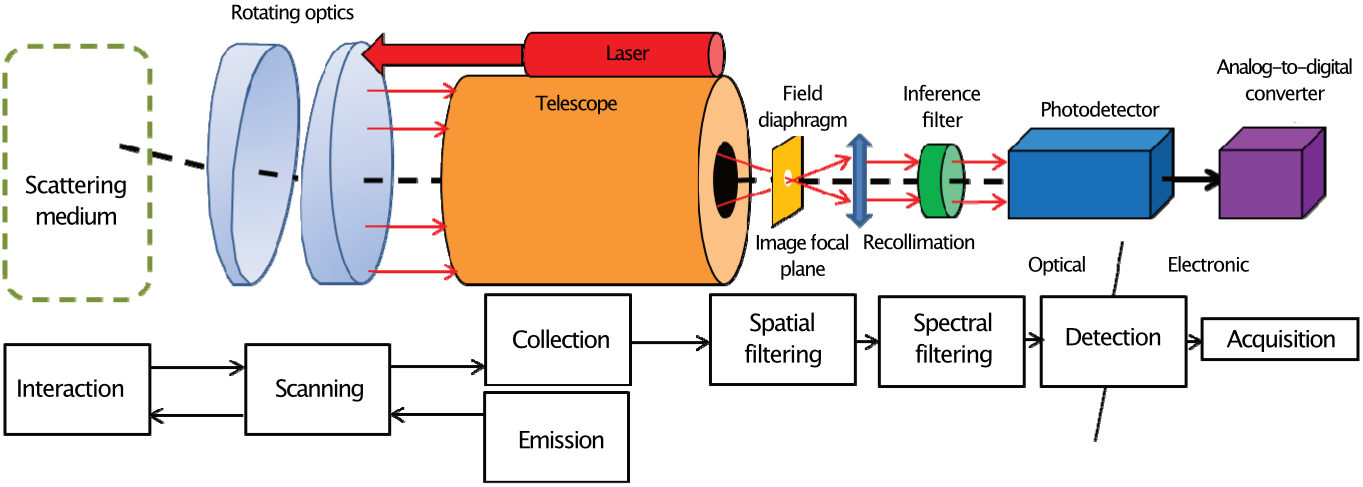
\includegraphics[width=\textwidth]{figs/lidar-components.png}
	\caption{Conventional architecture of a direct detection lidar system. Figure from \citet{Chazette16}.}%
\label{fig:lidar-components}
\end{figure}

In the optical part, a pulse of a particular wavelength (typically near-infrared) is generated by the laser source for each lidar measurement. 
It then passes through a set of  optics (lenses and mirrors) so that it leaves the scanner in an appropriate direction. 
After the pulse interacts with the scattering medium, it is reflected back into the scanning optics which then directs the signal into a telescope. 
The telescope converges the signal through a field diaphragm (essentially a tiny hole around the point of convergence). 
The field diaphragm blocks stray light rays (\eg\ sunlight reflected into the optics from any angle) from proceeding in the optical pipeline. 
Next, the light signal is recollimated so that it again consists only of parallel light rays. 
The final step of the optical part is the inference filter which blocks all wavelengths except for the wavelength of the laser source. 
This is again needed to block stray light rays from distorting the measurement.

The electronic part consists of a photodetector, which first transforms the light signal into an electrical current, which is then converted to a digital signal using the analogue-to-digital converter. 
Once the digital signal is available, further electronics can be used to interpret and record the signal.


%%%
\subsection{Laser wavelength}

Choosing the optimal laser wavelength is a compromise of several different factors. 
One needs to consider atmospheric scattering, 
\marginnote{atmospheric scattering}\index{atmospheric scattering}
\ie\ how much of the signal is lost simply by travelling through the atmosphere, and the absorption capacity of vegetation, \ie\ how much of  the signal is lost because it is absorbed by vegetation. In addition, there is the stray signal due to direct and scattered contributions of sunlight. While it is possible to filter such stray signals in the lidar system to some degree, it remains wise to choose a wavelength that is only minimally affected by it. Finally there are regulations that limit the laser radiance values permissible to the eye. This means that the power of emitted signal needs to be carefully controlled, and/or a wavelength must be chosen that  is not absorbed by the eye so much.

As a result, most lidar systems use a wavelength in the near-infrared spectrum, usually between 600 and 1000 nm. A notable exception is made for bathymetric purposes, in which case a green (532 nm) laser is used because that has a greater penetration ability in water.

\subsection{Scanning patterns}
In order to improve the capacity to quickly scan large areas, a number of rotating optical elements are typically present in a lidar system. Using these optical elements, \ie\  mirrors or prisms, the emitted laser pulse is guided in a cross-track direction (\ie\ perpendicular to the along-track direction in which  the aircraft moves, see Figure~\ref{fig:acqLidar}),  thereby greatly increasing the scanned ground area  per travelled meter of the aircraft.
Figure~\ref{fig:lidar-patterns} depicts a number of possible configurations of rotating optics and shows the resulting scanning patterns. It is clear that density of points on the ground is affected by the scanning pattern. The top example for example, yields much higher densities on edges of the scanned area. In practice more uniform patterns, such  as the bottom two examples are often preferred.

\begin{figure}
	\centering
	\includegraphics[width=0.7\textwidth]{figs/lidar-patterns.pdf}
	\caption{Different configurations of rotating mirrors and the associated scanning patterns from a moving platform. Arrows indicate the direction of the emitted laser signal. Figure from \citet{Chazette16}.}%
\label{fig:lidar-patterns}
\end{figure}



\begin{kaobox}[frametitle=\faExternalLink\ To read or to watch.]
	This YouTube video explains the principles of an aerial LiDAR system:
	\\
	\url{https://youtu.be/EYbhNSUnIdU}
\end{kaobox}


% TODO : put a side-by-side with vegetation and without lidar to show DTM and DSM


\section{Other acquisition techniques}%
\label{sec:acquisistion-techniques}

Apart from lidar there are also other sensor techniques that can be used to acquire elevation data. Some of these are  active sensors just like lidar (a signal is generated and emitted from the sensor), whereas others are passive (using the sun as light source). And like lidar, these sensors themselves only do range measurements, and need additional hardware such as a GPS receiver and an IMU to georeference the measurements. What follows is a brief description of the three other important acquisition techniques used in practice. 

% FIXME image with flight parameters and strips

\subsection{Photogrammetry}
\begin{marginfigure}
	\centering
	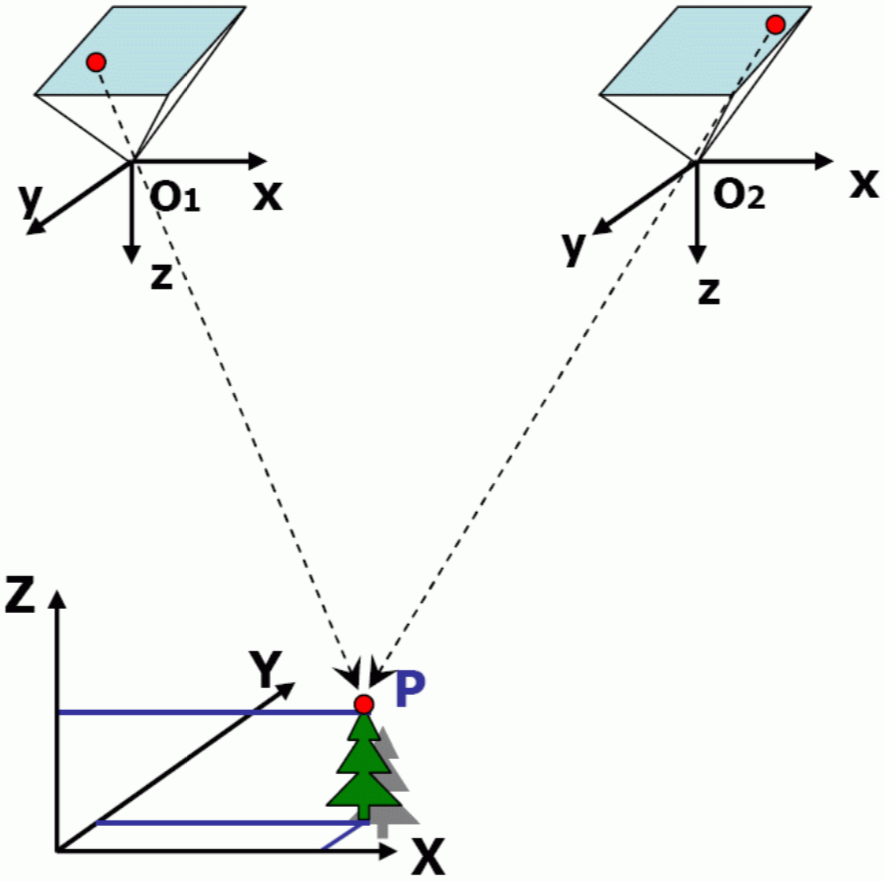
\includegraphics[width=\textwidth]{figs/photogrammetry.png}
	\caption{Photogrammetry}%
	\label{fig:acqPhoto}
\end{marginfigure}
Photogrammetry allows us to measure the distance from overlapping photographs taken from different positions. 
If a ground point, called a \emph{feature}, is identifiable in two or more images, its 3D coordinates can be computed in two steps. 
First, a viewing ray for that feature must be reconstructed for each image. 
A viewing ray can be defined as the line from the feature, passing through the projective centre of the camera, to the corresponding pixel in the image sensor (see Figure~\ref{fig:acqPhoto}). 
Second, considering that we know the orientation and position of the camera, the distance to the feature (and its coordinates) can be computed by calculating the spatial intersection of several viewing rays.

% interior orientation (camera parameters such as focal length) and the exterior orientation (camera position and orientation)

The number of 3D point measurements resulting from photogrammetry thus depends on the number of features that are visible in multiple images, \ie\ the so-called matches.
With \emph{dense image matching} 
\marginnote{dense image matching}\index{dense image matching}
it is attempted to find a match for every pixel in an image. 
If the ground sampling distance, \ie\ the pixel size on ground level, is small (around 5cm for state-of-the-art systems), point densities of hundreds of points per square meter can be achieved, which is much higher than the typical lidar point cloud (typically up to dozens of points per square meter). 

In photogrammetry we distinguish between \emph{nadir} images, 
\marginnote{nadir images}\index{nadir images}
that are taken in a direction straight down from the camera, and \emph{oblique}
\marginnote{oblique images}\index{oblique images}
images that are taken at an angle with respect to the nadir direction.
Vertical features such as building façades are only visible on oblique images.
Therefore, oblique images are needed if one wants to see building façades in a dense image matching point cloud.

Because photography is used, photogrammetry gives us also the colour of the target surface, in addition to the elevation.
This could be considered an advantage over lidar which captures several attributes for each point (\eg\ the intensity of measured laser pulse and the exact GPS time of measurement), but colour is not among them.

Both airborne and spaceborne photogrammetry are possible.

%%%
\subsection{InSAR}

Interferometric synthetic aperture radar (InSAR) is a radar-based technique that is used from space in the context of terrain generation. 
It is quite different from airborne lidar or photo\-gramme\-try-based acquisition because of the extremely high altitude of the satellite carrying the sensor. 
Signals have to travel very long distances through several layers of unpredictable atmospheric conditions. 
As a result the speed of the radar signal is not known and the time-of-flight principle can not be used to get detailed measurements. 
However, by using a comprehensive chain of processing operations based on the measured phase shifts and the combination of multiple InSAR images, accurate elevation can still be measured. 
With InSAR it is possible to cover very large regions in a short amount of time, \eg\ the global SRTM\footnote{\url{https://en.wikipedia.org/wiki/Shuttle_Radar_Topography_Mission}} dataset was generated with InSAR\@. 
Compared to dense image matching and lidar, InSAR-derived DTMs usually have a much lower resolution, \eg\ SRTM has a pixel size of 30 meters.

%%
\begin{kaobox}[frametitle=\faExternalLink\ To read or to watch.]
	\href{https://en.wikipedia.org/wiki/Interferometric_synthetic-aperture_radar}{Wikipedia page about \emph{Interferometric synthetic-aperture radar}}.
\end{kaobox}


%%%
\subsection{Echo sounding}%
\label{sec:mbes}
Echo sounding is a form of sonar that can be used for bathymetry, \ie\ mapping underwater terrains from a boat. 
Similar to lidar, it uses the time-of-flight principle to compute distance, but sound is used instead of light. 

Single-beam and multi-beam echo sounders exist. Multi-beam systems are capable of receiving many narrow sound beams from one emitted pulse. As a result it measures the target surface much more accurately. 
For bathymetry usually a multi-beam echo sounder is used.

Chapter~\ref{chap:bathymetry} describes techniques to process bathymetric datasets and create terrain of the seabed.

%%
\begin{kaobox}[frametitle=\faExternalLink\ To read or to watch.]
  The principles of echo sounding.
  \\
  \url{https://en.wikipedia.org/wiki/Echo_sounding}
\end{kaobox}




\section{Artefacts}%
\label{sec:artefacts}

In the acquisition process, there are many aspects---both under our control and not under our control--- that affect the quality and usability of the resulting elevation data for a given application. 
Some examples are
\begin{itemize}
	\item the choice of the sensor technique, 
	\item the sensor specifications, \eg\ the resolution and focal length of a camera, or the scanning speed, the width of the swath, and scanning pattern of a lidar system,
	\item the flight parameters, \eg\ the flying altitude and the distance and overlap between adjacent flights,
	\item atmospheric conditions, 
	\item the physical properties of the target surface.
\end{itemize}

An artefact is any error in the perception or representation of information that is introduced by the involved equipment or techniques. 
Artefacts can result in areas without any measurements (\eg\ the \emph{no-data} values in a raster), or in so-called \emph{outliers}, \ie\ sample points with large errors in their coordinates. 
\marginnote{outliers}\index{outliers}

We distinguish three types of artefacts, 
\begin{enumerate}
	\item those that occur due to problems in the sensor, 
	\item those that occur due to the geometry and material properties of the target surface, 
	\item those that occur due to post-processing steps.
\end{enumerate}

% Active/passive sensors
% different platforms ground/airborne/space
% different physical principles
% pulse footprint, wavelength
% different sensor specs (resolution, speed) and operation specs (flight height etc)
% different cost, update cycles

\subsection{Sensor orientation}
The sensor position and orientation are continuously monitored during acquisition, \eg\  by means of GNSS and an IMU for airborne and seaborne systems, and used to determine the 3D coordinates of the measured points. 
Consequently, any errors in the position and orientation of the sensor platform affect the elevation measurements. 
For this reason adjacent flight strips (see Figure~\ref{fig:lidarStrips}) often need to be adjusted to match with each other using ground control points. 
\begin{figure}
	\centering
	\begin{subfigure}{0.4\linewidth}
		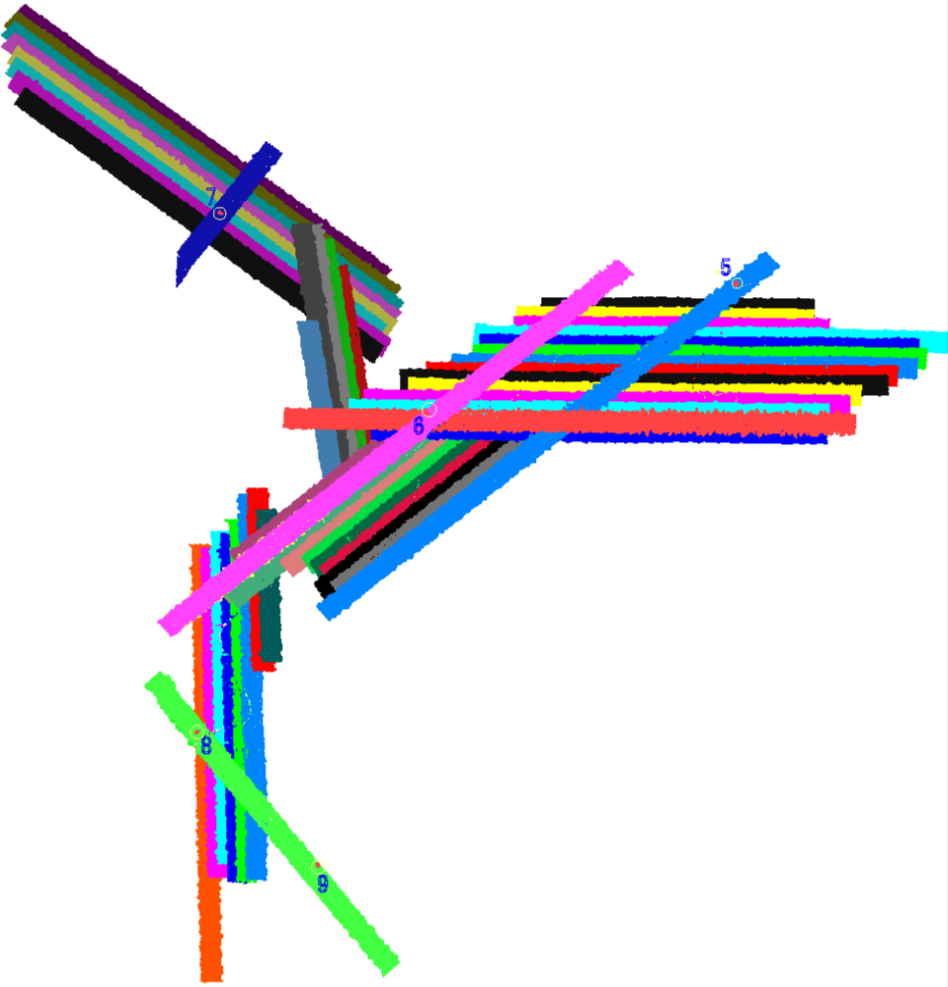
\includegraphics[width=\textwidth]{figs/lidar_strips.png}
		\subcaption{Plan view of the different strips of a lidar survey \citep{Kornus03}}\label{fig:lidarStrips}
	\end{subfigure}
	\quad
	\begin{subfigure}{0.4\linewidth}
		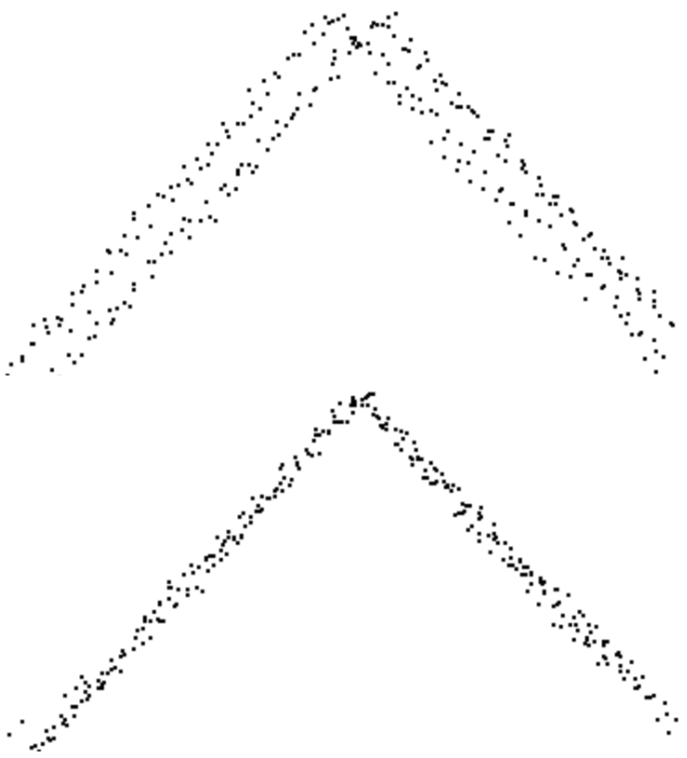
\includegraphics[width=\textwidth]{figs/strip_adjustment.png}
		\subcaption{Cross-section of gable roof before (top) and after (bottom) strip adjustment \citep{Vosselman02}}\label{fig:lidarGableRoof}
	\end{subfigure}
	\caption{Strip adjustment for lidar point clouds}%
\label{fig:lidarStripAdj}
\end{figure}
If the strip adjustments process fails or is omitted, a `ghosting' effect can occur as illustrated in Figure~\ref{fig:lidarGableRoof} (top). 
Photogrammetry knows a similar process called aerial triangulation, in which camera positions and orientation parameters (one set for each image) are adjusted to fit with each other. Errors in the aerial triangulation can lead to a noisy result for the dense matching as seen in Figure~\ref{fig:dim}.
\begin{figure}
	\centering
	\begin{subfigure}{0.95\linewidth}
		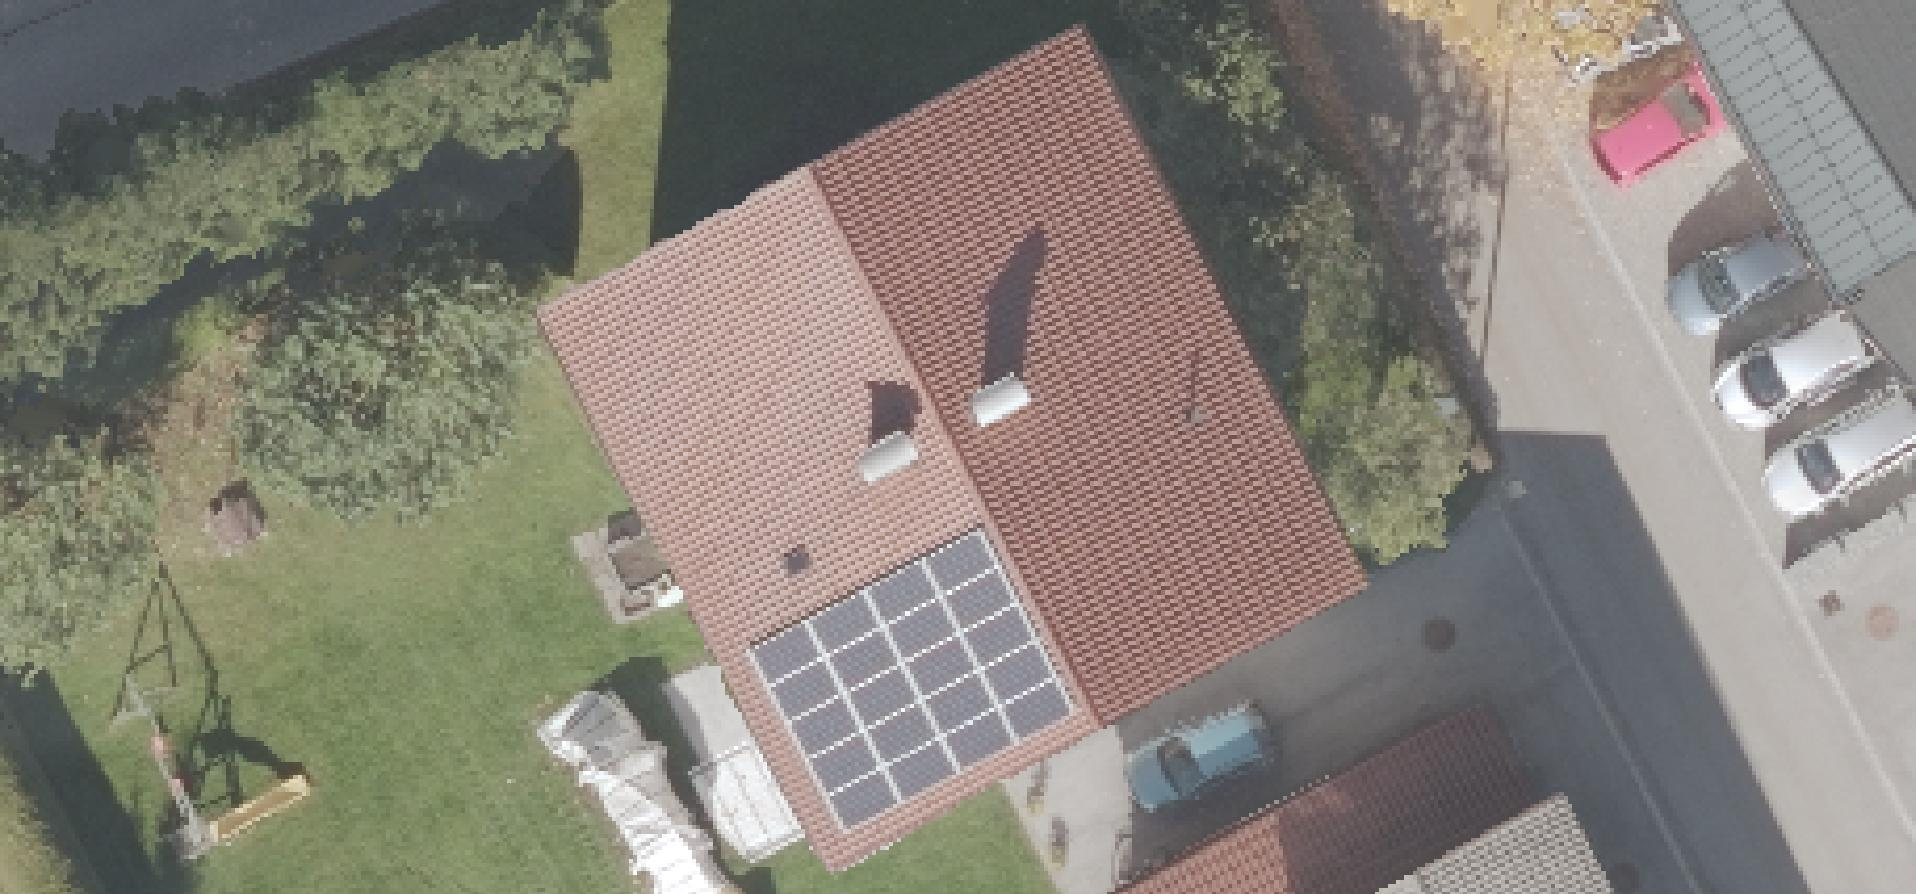
\includegraphics[width=\textwidth]{figs/Roof_OP_NA_10cm.jpg}
		\subcaption{Nadir image}\label{fig:dim:a}
	\end{subfigure}
	
	\begin{subfigure}{0.95\linewidth}
		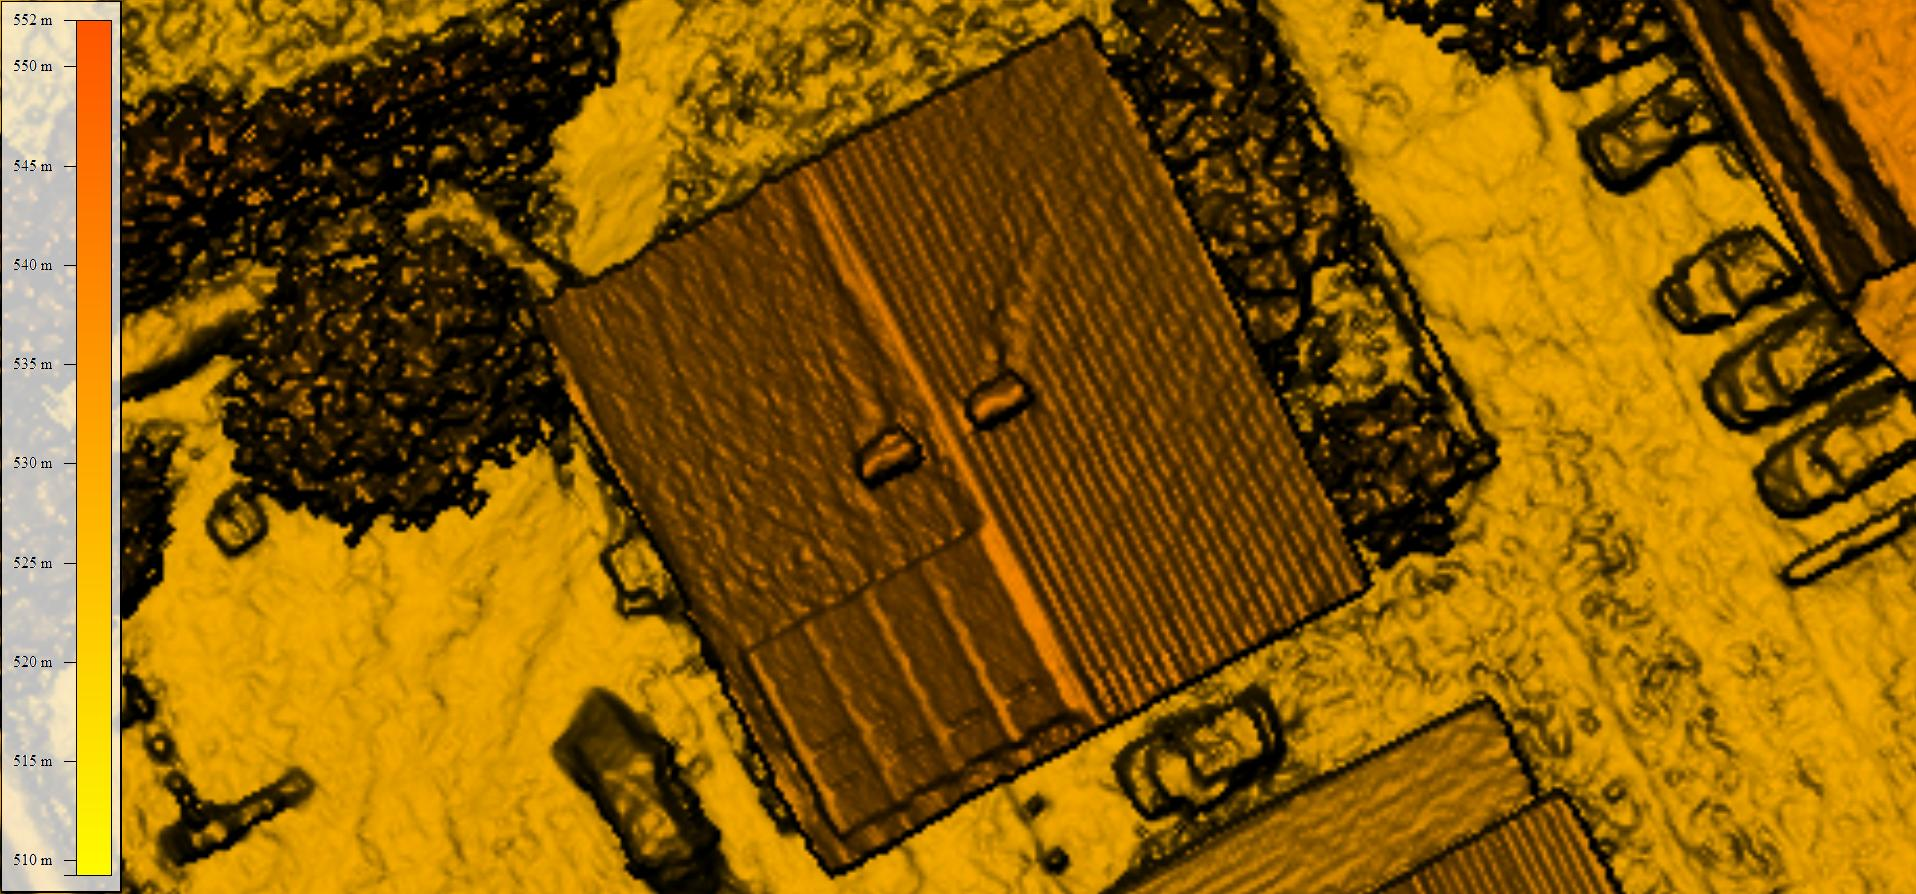
\includegraphics[width=\textwidth]{figs/Roof_DSM_NA_10cm.jpg}
		\subcaption{DSM with good aerial triangulation}\label{fig:dim:b}
	\end{subfigure}
	\begin{subfigure}{0.95\linewidth}
		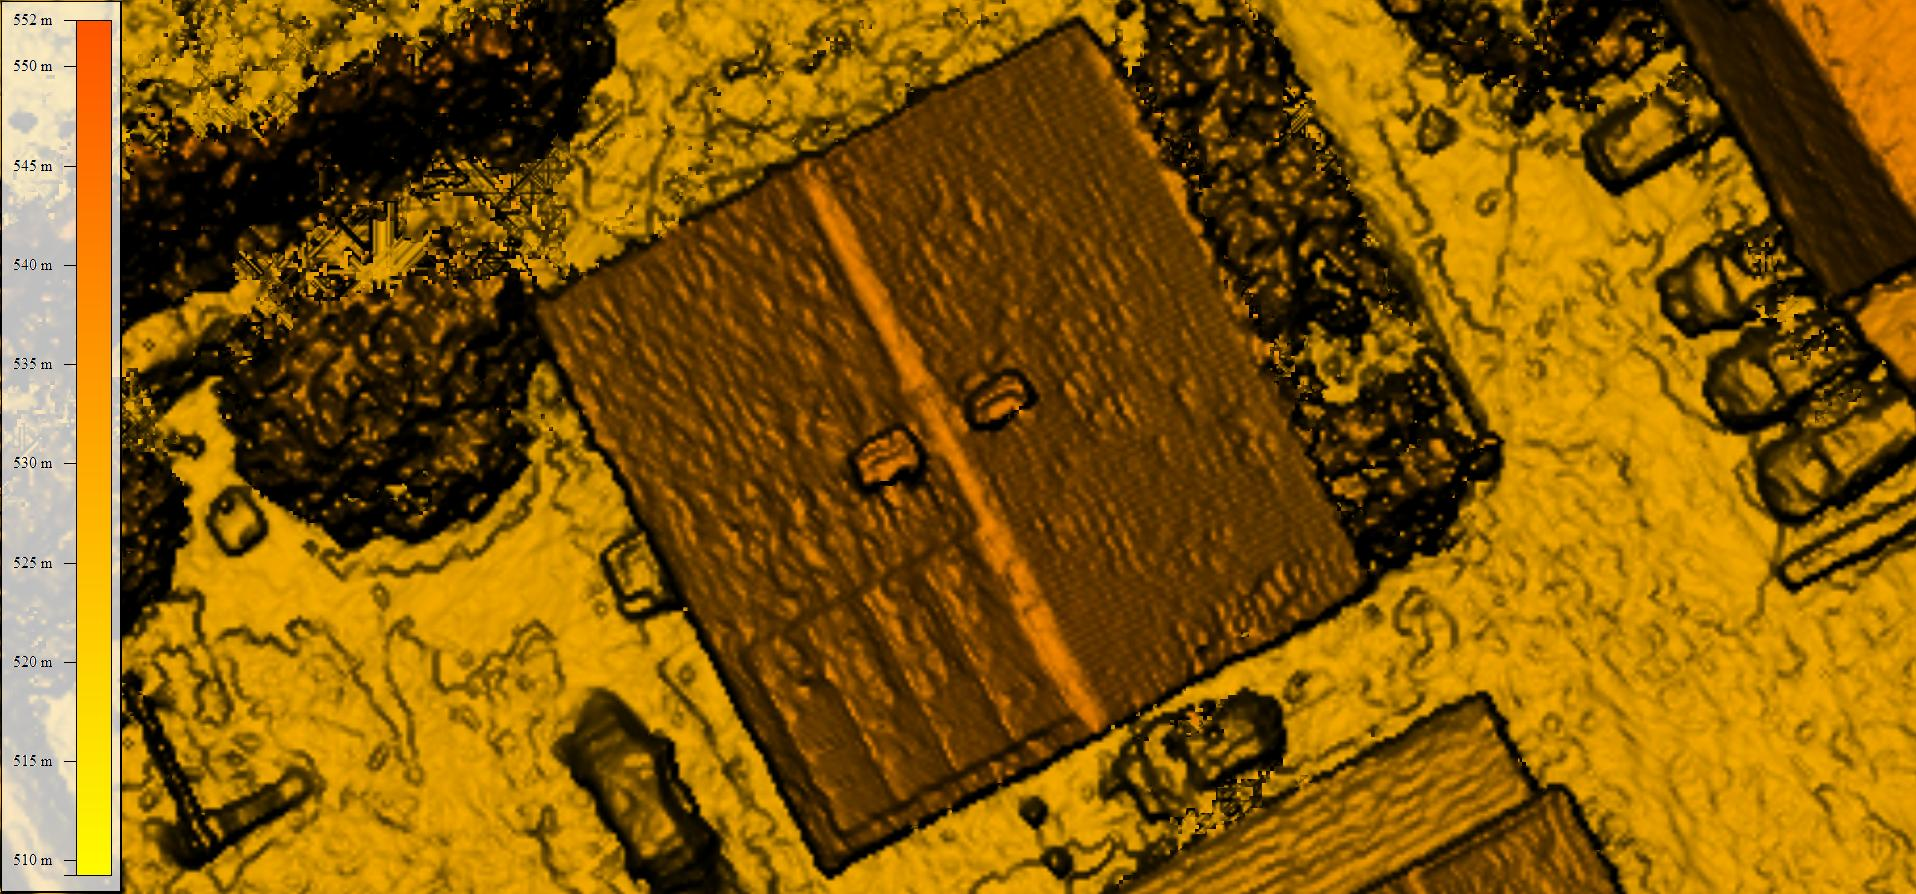
\includegraphics[width=\textwidth]{figs/Roof_DSM_NA+OBL_10cm.jpg}
		\subcaption{DSM with poor aerial triangulation}\label{fig:dim:c}
	\end{subfigure}
	\caption{Errors in aerial triangulation can lead to distortions in the DSM (derived from dense image matching). Images courtesy of Vermessung AVT.}%
\label{fig:dim}
\end{figure}


\subsection{Target surface}
Many commonly occurring  artefacts  happen due to properties of the target surface. We distinguish three classes.

\subsubsection{Geometry} 
The shape of the target surfaces in relation to the sensor position has a great effect on 1) local point densities and 2) occlusion. As you can see from Figure~\ref{fig:lidarAcquisitionConditions:a},
\begin{marginfigure}
	\centering
	\includegraphics[width=\textwidth,page=2]{figs/lidarAcq.pdf}
	\caption{Point distribution and occlusion}%
	\label{fig:lidarAcquisitionConditions:a}
\end{marginfigure}
which illustrates this for lidar, surfaces that are closest to the scanner and orthogonal to the laser beams will yield the highest point densities (see the rooftop of the middle house). Very steep surfaces on the other hand, yield relatively low point densities (see the façades of the buildings). 

\index{occlusion}
\emph{Occlusion} happens when a surface is not visible from the scanner position. 
As a result there will be gaps in the point coverage, also visible in Figure~\ref{fig:lidarAcquisitionConditions:a}. 
Notice how some steep surfaces and some of the adjacent ground are not registered at all by the scanner because it simply could not `see' these parts.

The severity of both effects mostly depends on the geometry of the target objects and flight parameters such as the flying altitude and the amount of overlap between flight strips.
However, regardless of what flight parameters are chosen for a survey both effects are almost always visible somewhere in the resulting dataset, see for example Figure~\ref{fig:pcd} for different lidar datasets for the same area.

% oblique vs nadir for occlusion
%Especially occlusion can be a problem for (2.5D) DTM generation because it causes no-data areas that may be problematic.

\begin{figure*}
	\centering
	\begin{subfigure}{0.45\linewidth}
		
\includegraphics[width=\textwidth]{figs/ahn1_d.png}
		\subcaption{AHN1 (1996-2003)}\label{fig:pcd:ahn1}
	\end{subfigure}
	\quad
	\begin{subfigure}{0.45\linewidth}
		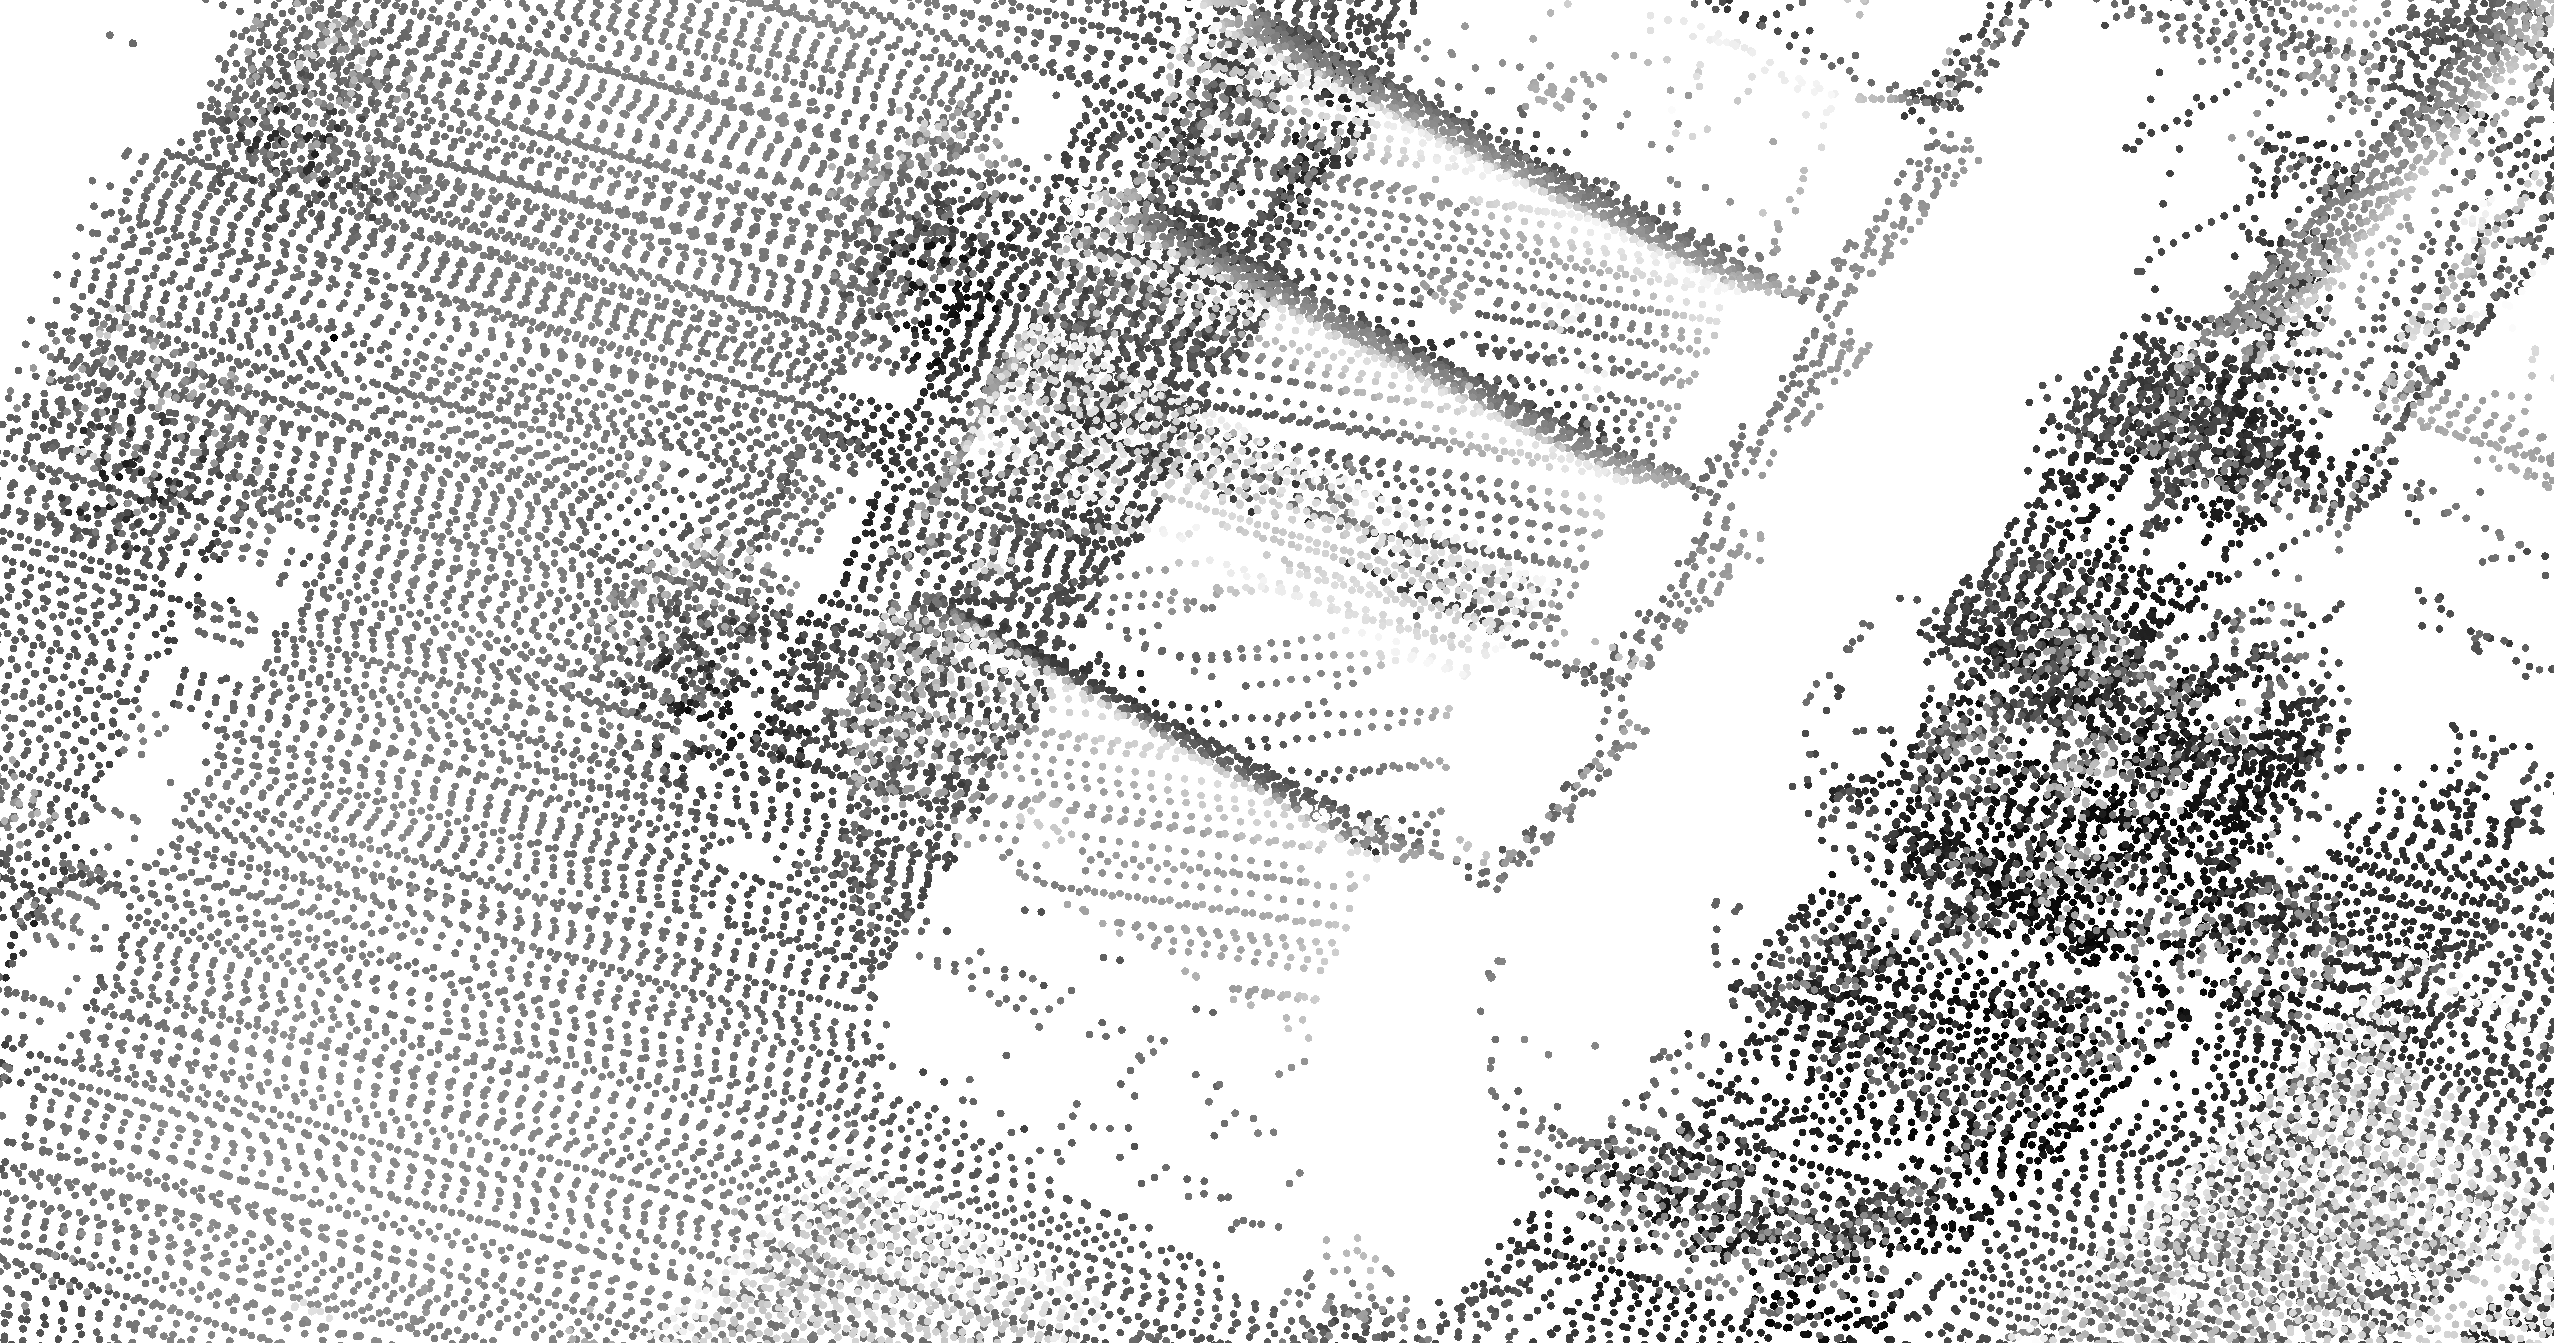
\includegraphics[width=\textwidth]{figs/ahn2_d.png}
		\subcaption{AHN2 (2008)}\label{fig:pcd:ahn2}
	\end{subfigure}
	
	\begin{subfigure}{0.45\linewidth}
		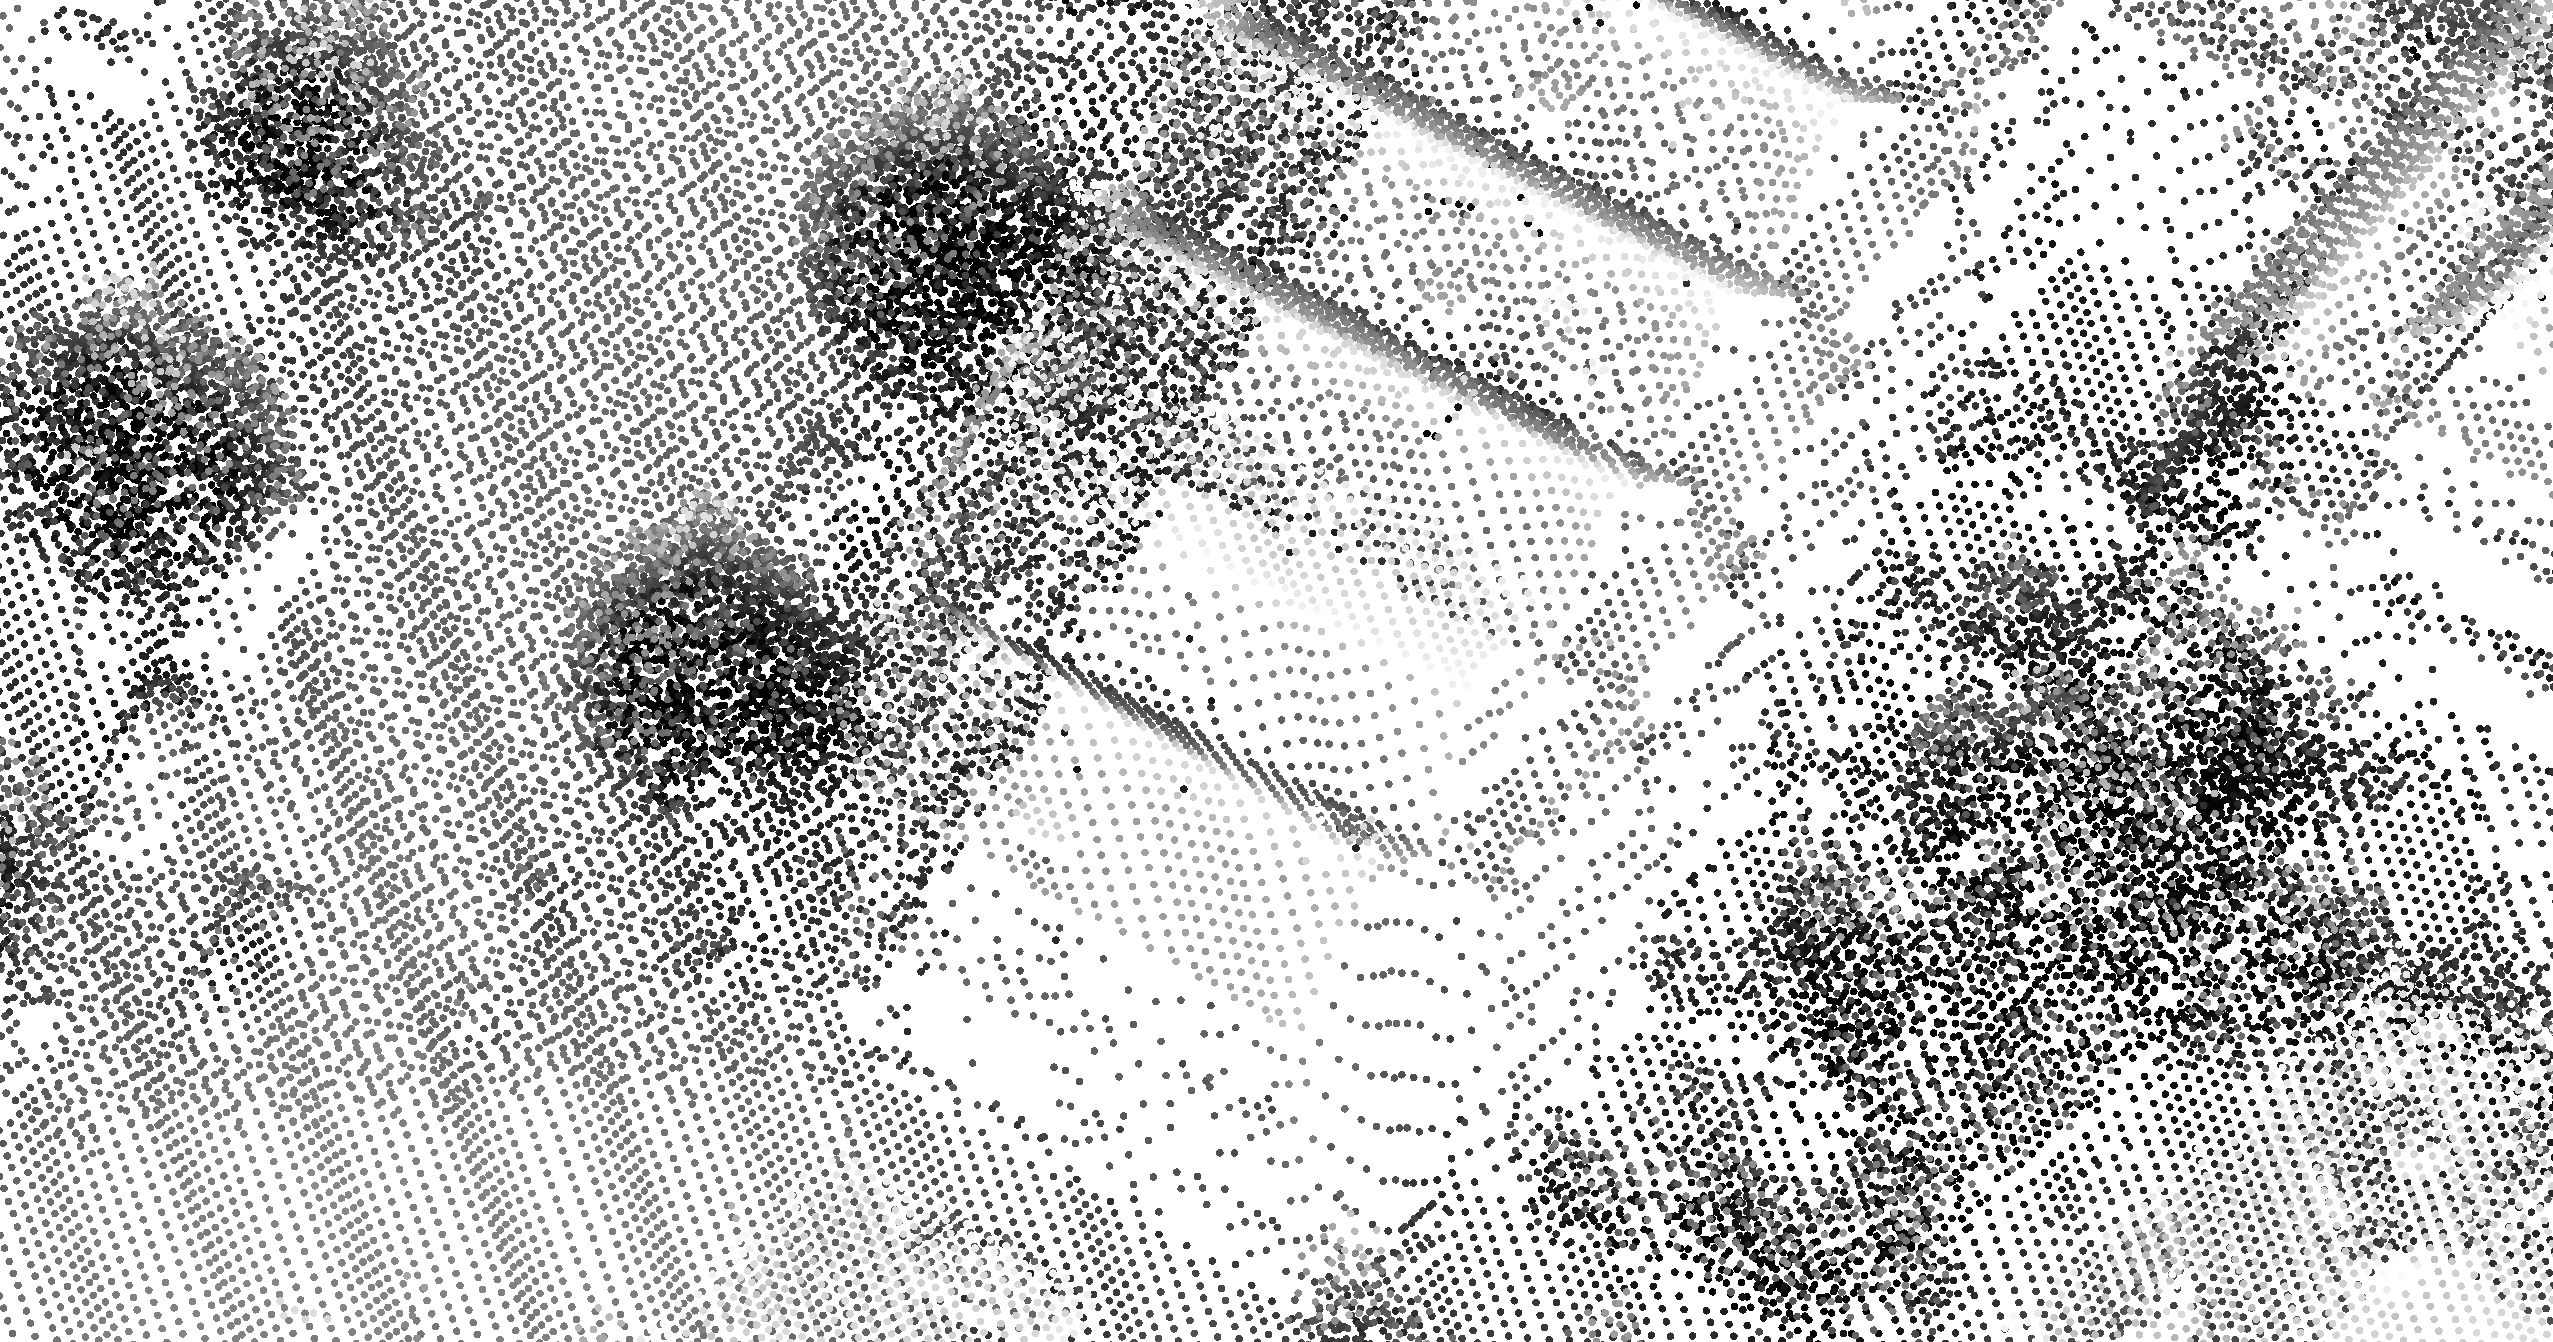
\includegraphics[width=\textwidth]{figs/ahn3_d.png}
		\subcaption{AHN3 (2014)}\label{fig:pcd:ahn3}
	\end{subfigure}
	\quad
	\begin{subfigure}{0.45\linewidth}
		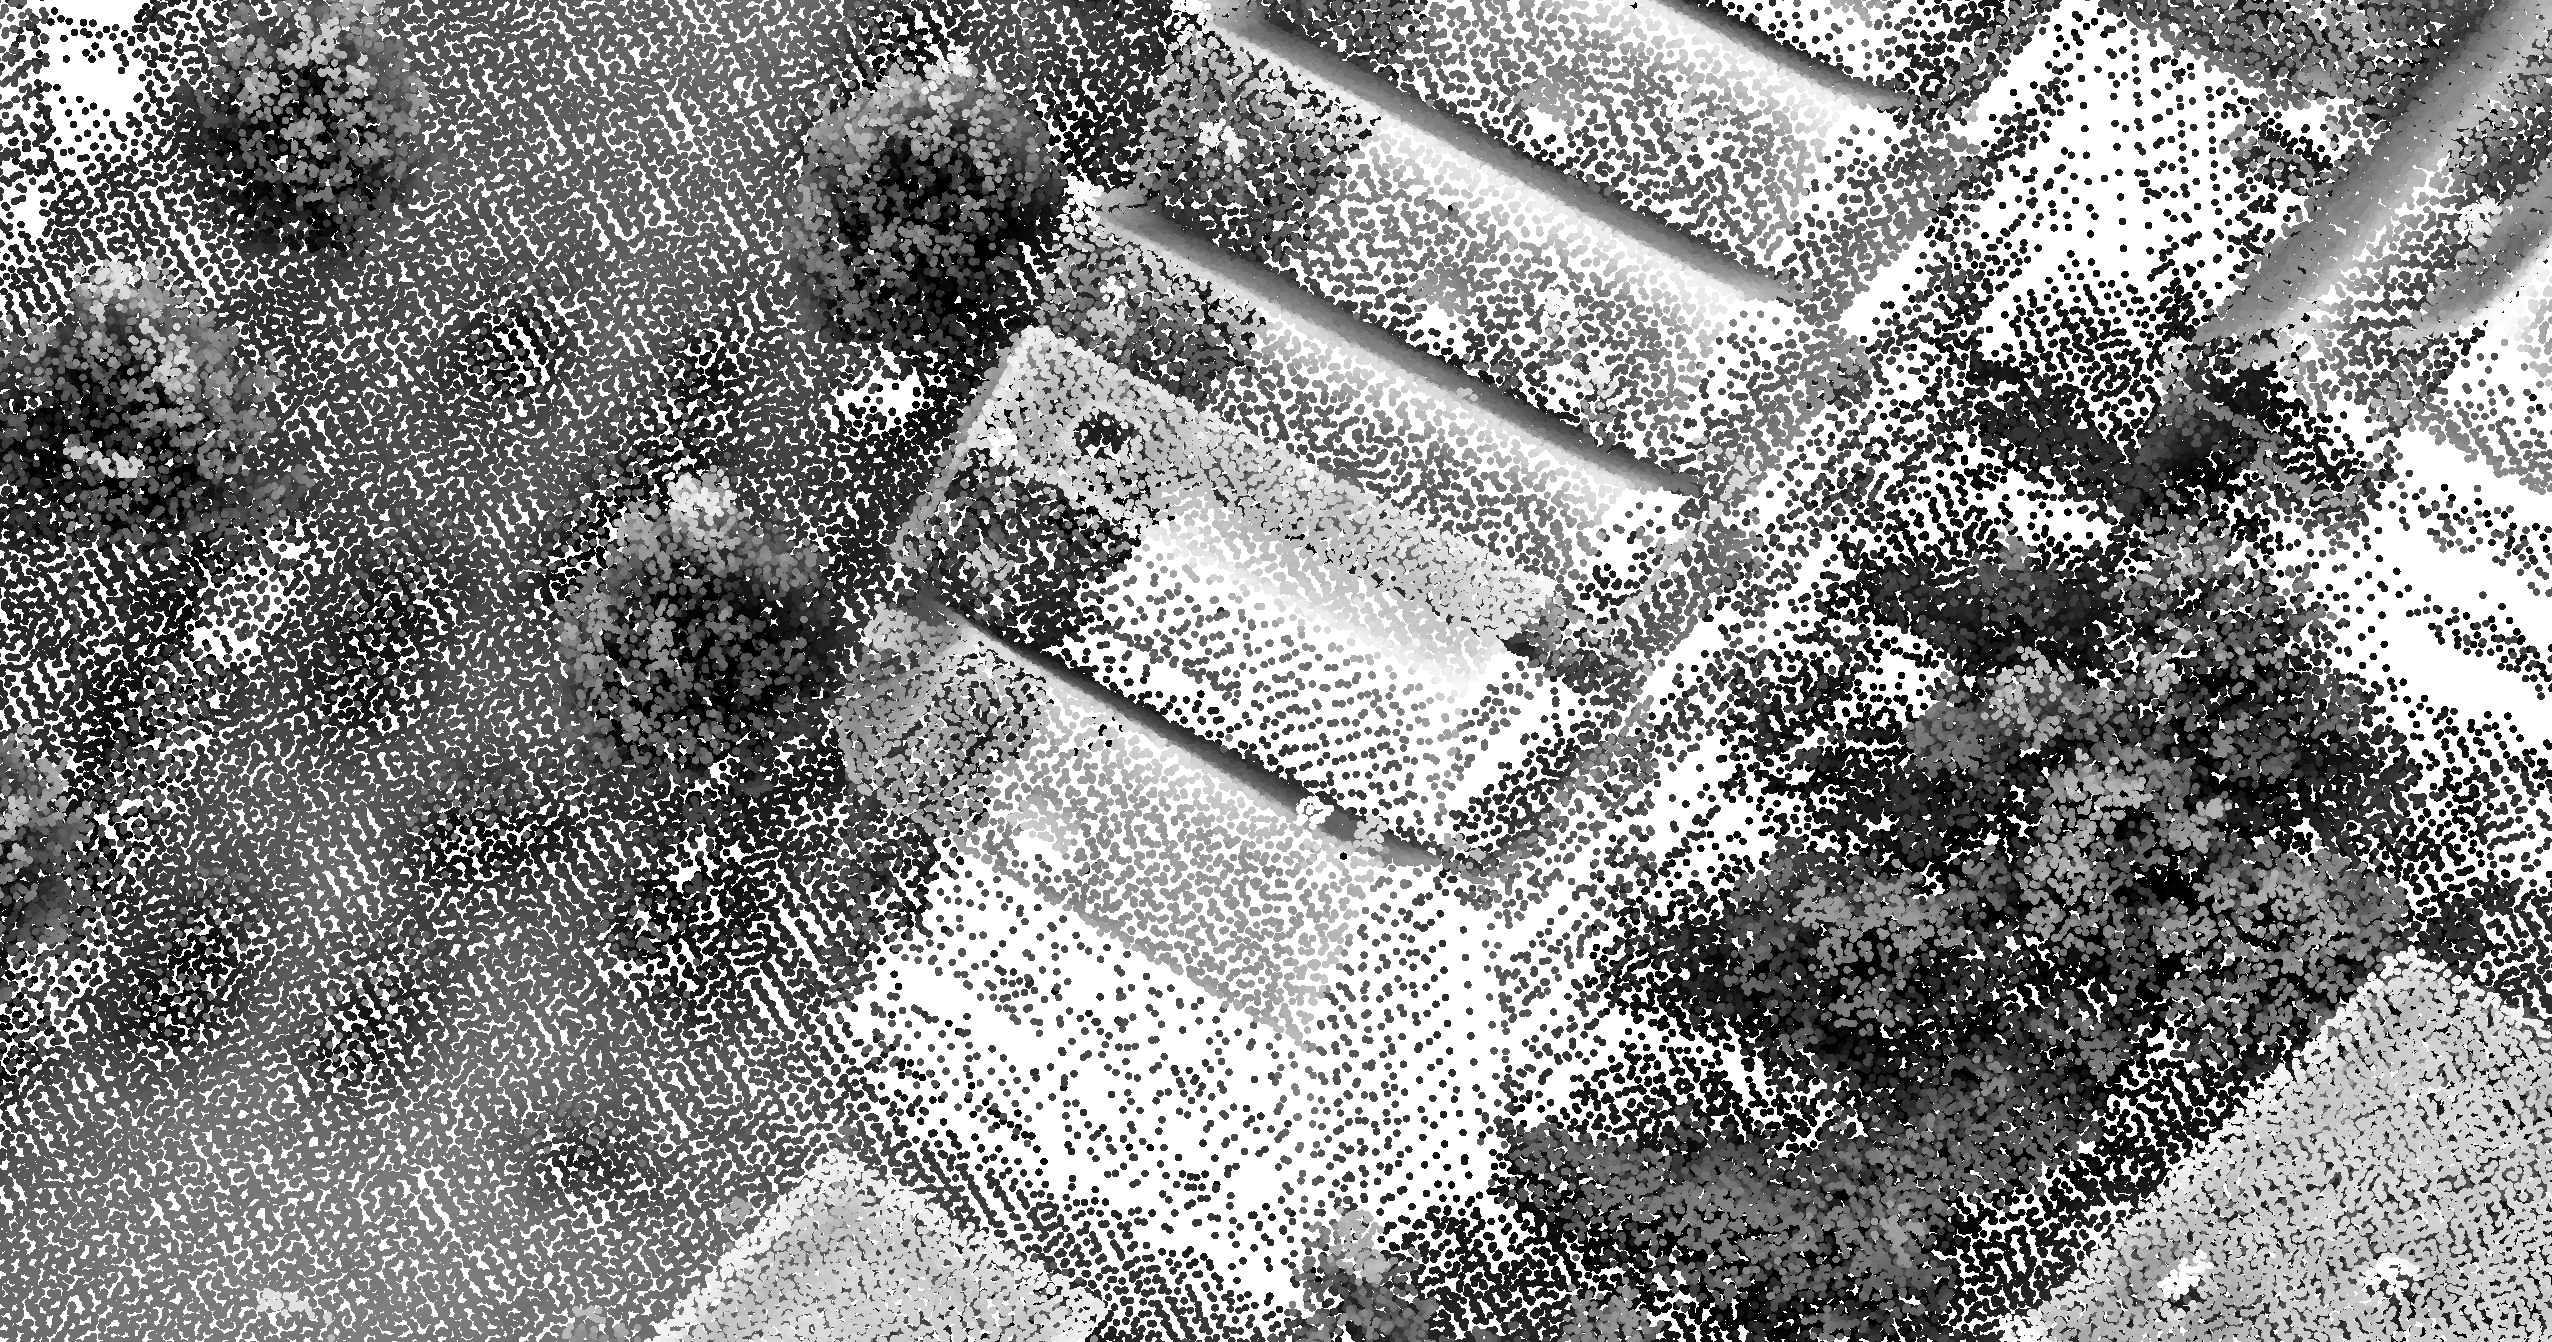
\includegraphics[width=\textwidth]{figs/rdam16_d.png}
		\subcaption{City of Rotterdam (2016)}\label{fig:pcd:rdam16}
	\end{subfigure}
	\caption{Several lidar point clouds for the same area in the city of Rotterdam. Point distribution and occlusion effects vary.}%
\label{fig:pcd}
\end{figure*}

\subsubsection{Material properties}
Depending on material properties of a target surface, signals may be reflected in a way that makes it impossible to compute the correct distance. 
Surfaces that act like a mirror are especially problematic, Figure~\ref{fig:lidarAcquisitionConditions:b} illustrates this. 
\begin{marginfigure}
	\centering
	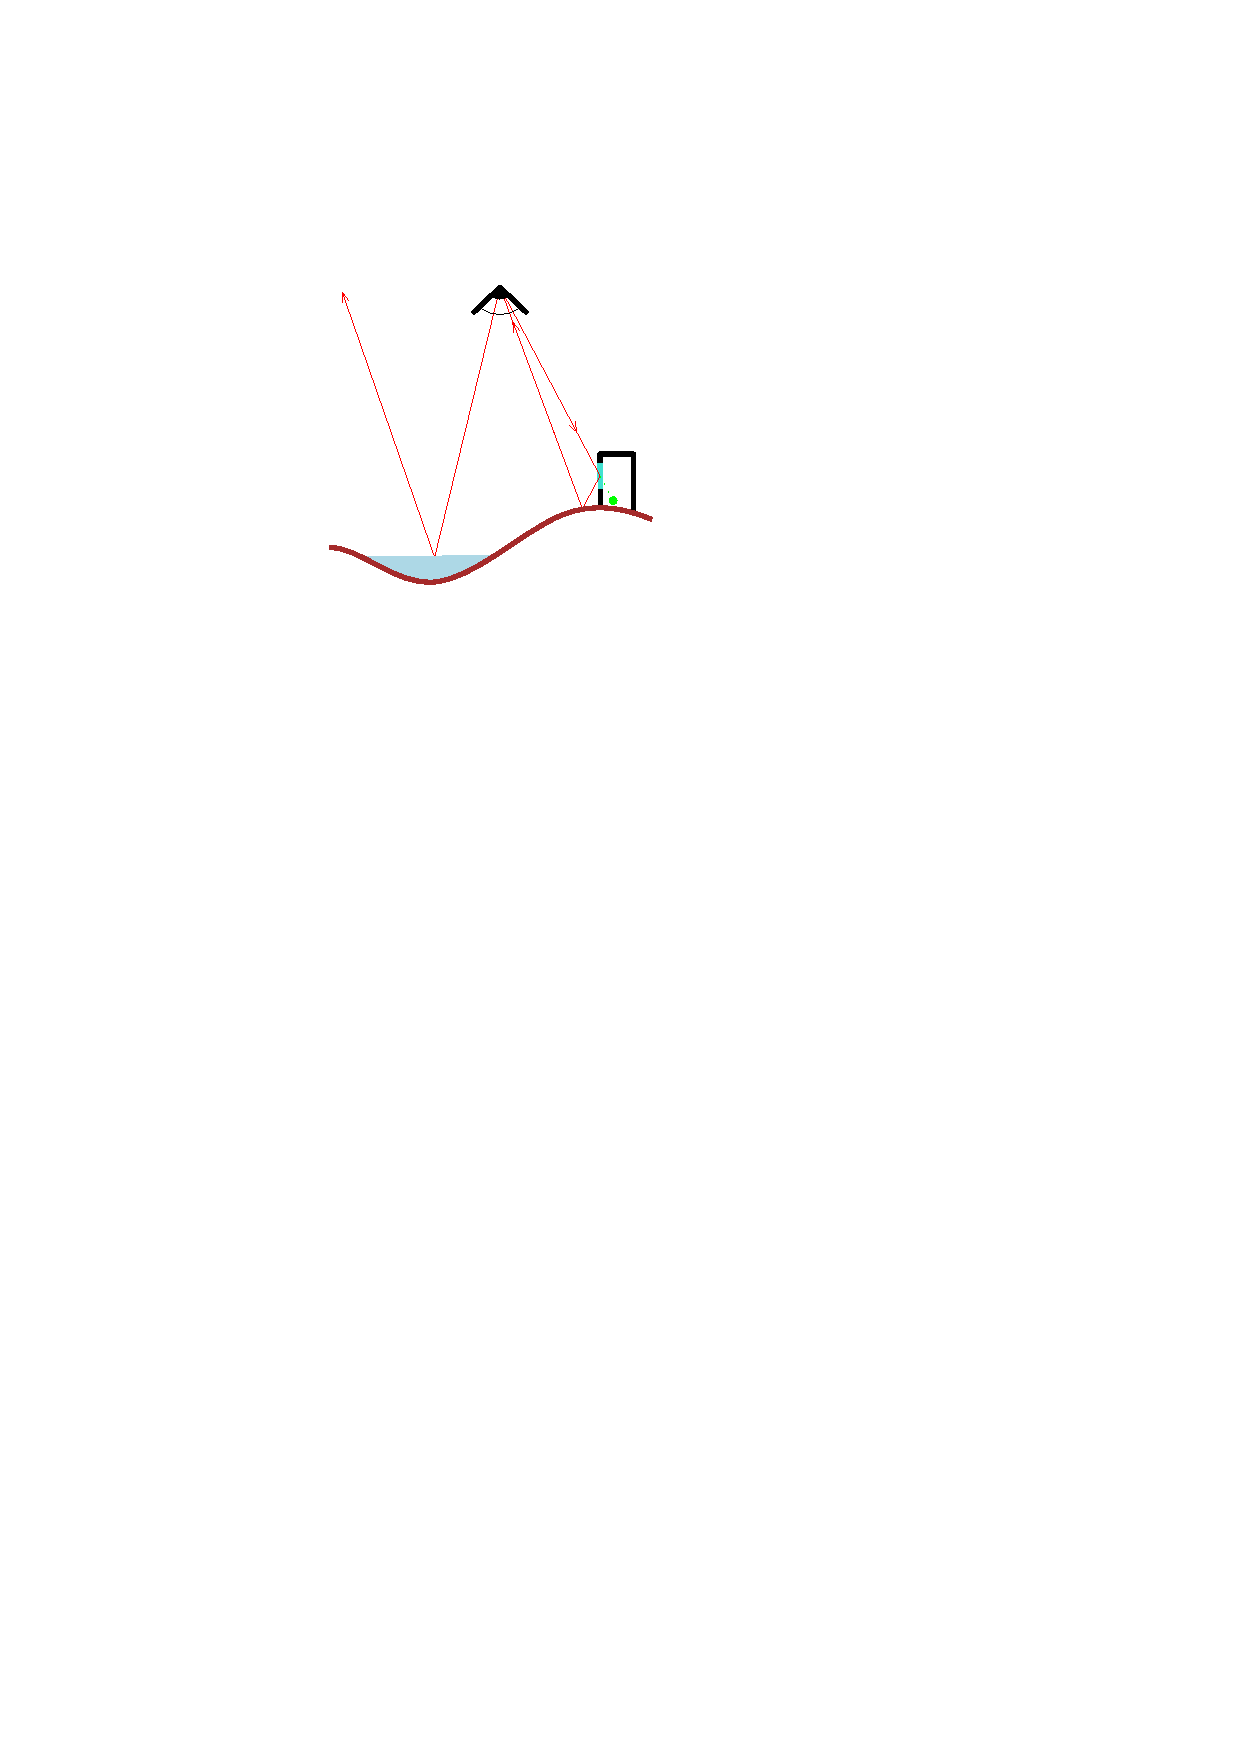
\includegraphics[width=\textwidth,page=1]{figs/lidarAcq.pdf}
	\caption{Reflection and multi-path}%
	\label{fig:lidarAcquisitionConditions:b}
\end{marginfigure}
First, it may happen that a pulse is reflected away from the sensor, \eg\ from a water surface, resulting in no distance measurement for that pulse. 
Or, in the case of photogrammetry, we will observe a different reflection in each image which heavily distorts the matching process, sometimes resulting in extreme outliers for water surfaces.  
In some cases, and only for active sensors, the reflected pulse does make its way back to the sensor, see for example the right half of Figure~\ref{fig:lidarAcquisitionConditions:b}. 
However, it will have travelled a longer distance than it should have and the scanner only knows in which direction it emitted the pulse. 
This effect is called \emph{multi-path} and the result is that points are measured at a distance that is too long and therefore they show up below the ground surface in the point cloud (see Figure~\ref{fig:outliers}).  
\begin{figure}
	\centering
	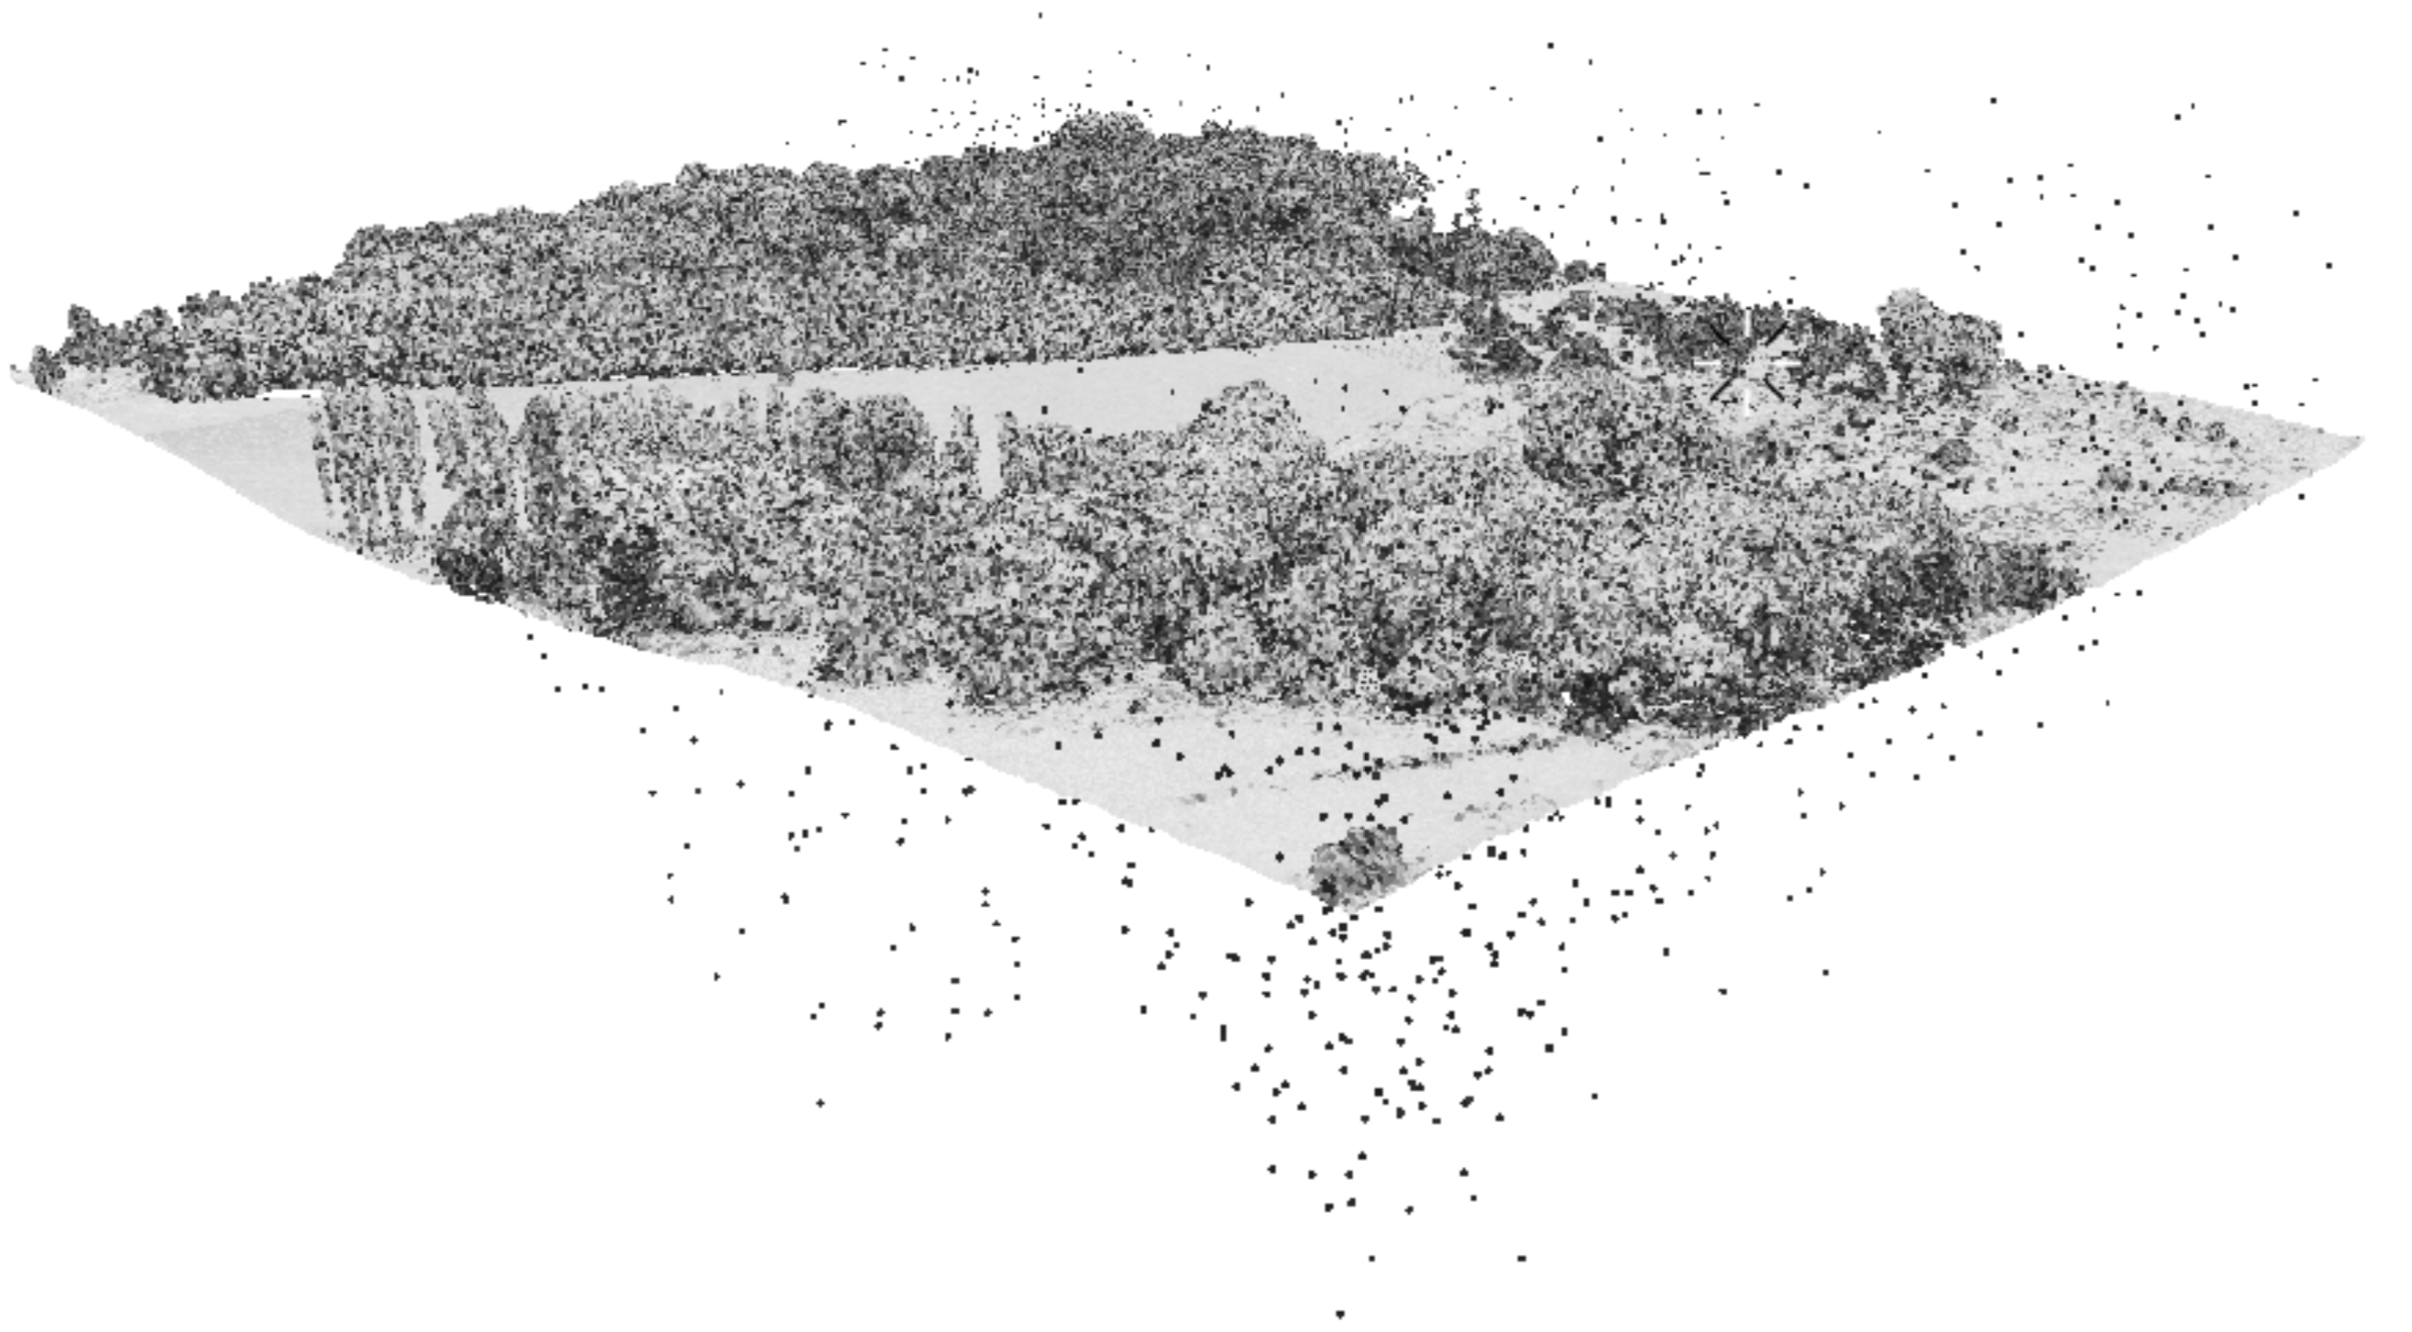
\includegraphics[width=\textwidth]{figs/outliers.png}
	\caption{Outliers, below and above the ground, in a lidar point cloud dataset.}%
\label{fig:outliers}
\end{figure}

Photogrammetry suffers from a few other problems as well, such as surfaces that have a homogeneous texture that make it impossible to find distinguishing features that can be used for matching. 
This may also happen in poor lightning conditions, for example in the shadow parts of an image.
%no texture (shadow), multi-path, complete absorption lightning conditions: shadow poor matching

\subsubsection{Moving objects}
An example of moving objects are flocks of birds flying in front of the scanner. These can cause outliers high above the ground, as illustrated in Figure~\ref{fig:outliers}.


\subsection{Processing}
It is common to perform some kind of process after acquisition in order to fix errors caused by the reasons mentioned above. 
In most cases such processes are largely successful. 
For instance, one can attempt to fill the void regions, sometimes referred to as \emph{no-data} regions, that are for instance due to pools of rainwater or occlusion, using an interpolation method (Figure~\ref{fig:voidfill}).
\begin{figure}
	\centering
	\begin{subfigure}{0.9\linewidth}
		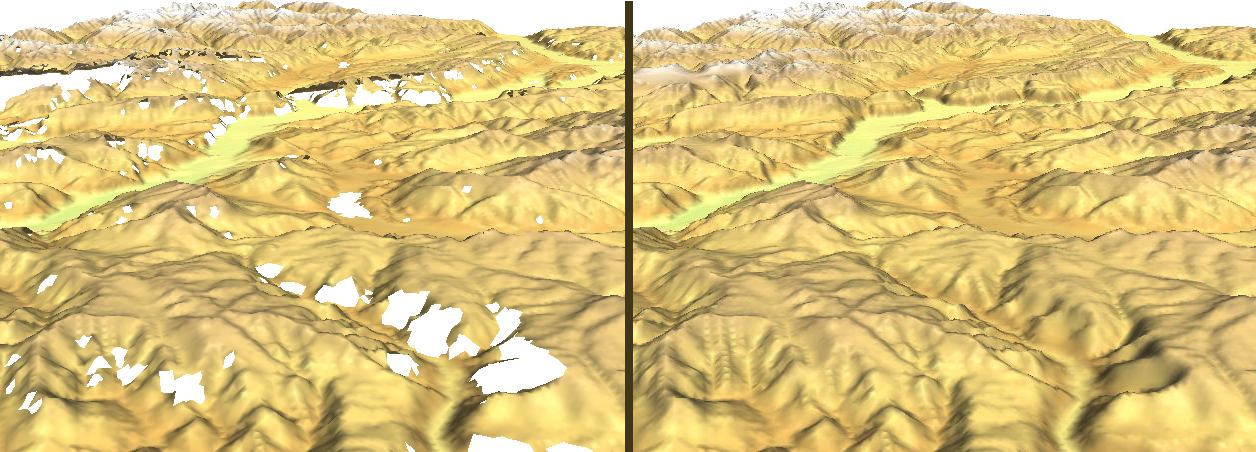
\includegraphics[width=\textwidth]{figs/srtm_trento_voidfill.png}
		\subcaption{Void-filling through interpolation in SRTM data}\label{fig:voidfill}
	\end{subfigure}
	\begin{subfigure}{0.9\linewidth}
		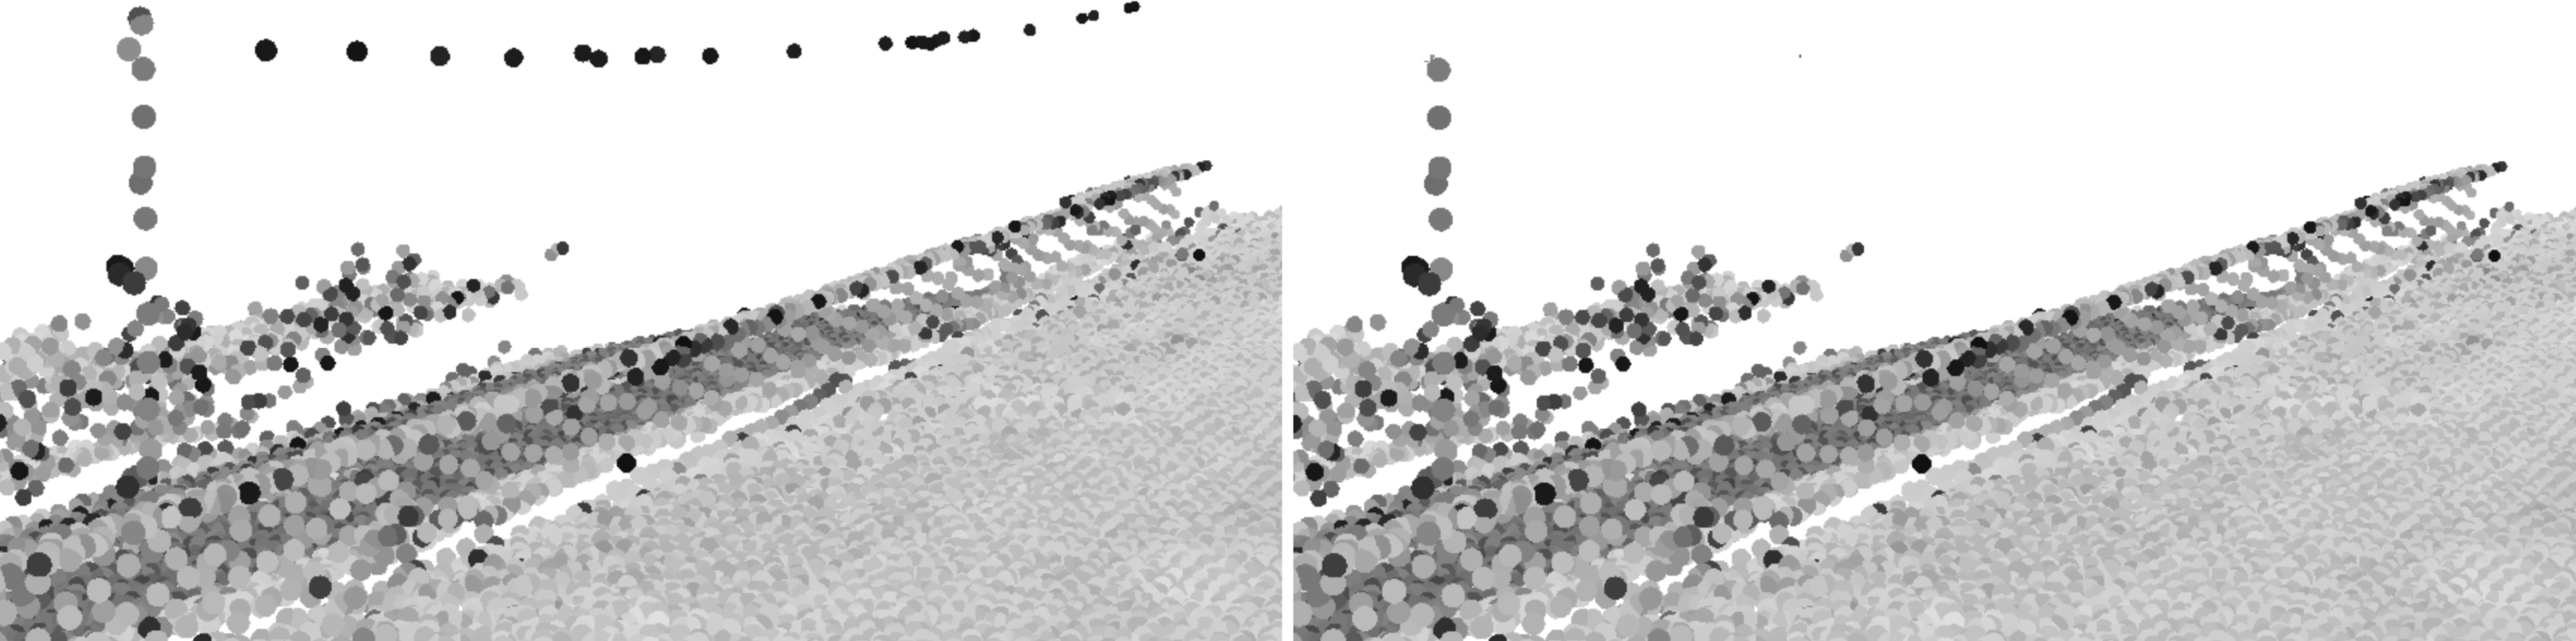
\includegraphics[width=\textwidth]{figs/ourlier-detection-wrong.png}
		\subcaption{Good points, \ie\ those on the power line, may be removed during outlier detection}		\label{fig:outlier-wrong}
	\end{subfigure}
	\caption{Post-processing aimed at correcting artefacts. Before processing (left) and after processing (right).}%
	\label{fig:processing}
\end{figure}
Or, one can attempt to detect and remove outliers caused \eg\ by multi-path effects or flocks of birds\footnote{This is a topic of lesson 12}. 
However, while the intention is always to reduce the number and severity of artefacts, these processes sometimes introduce distortions of their own.
For example, an outlier detection algorithm may remove `good' points if they look the same as outliers to the outlier detection algorithm (see \eg\ Figure~\ref{fig:outlier-wrong}).
And void-filling is only effective if the void area is not too large, since interpolation methods always assume there is sufficient neighbourhood information to work with\footnote{Chapters~\ref{chap:interpol} and~\ref{chap:kriging} explore the topic of spatial interpolation in detail.}.


%%
\begin{kaobox}[frametitle=\faExternalLink\ To read or to watch.]
This is a paper that compares lidar and photogrammetry derived point clouds for the generation of a DEM\@. It shows that even when artefacts seem to be under control, both techniques may measure different elevations 

\fullcite{Ressl16}
\textbf{PDF:} \url{https://3d.bk.tudelft.nl/courses/geo1015/data/others/Ressl16.pdf}
\end{kaobox}

%For instance, an outlier filter 
%misclassified points, smoothing effects in DIM

%Difficulties in automated DTM generation
%• Homogeneous areas and repeating structures;
% No distinct peak or multiple peaks of the similarity measures
%• Areas occluded in one image
% No correspondence exists;
%• Steep sloped surfaces
% Geometric difference between template and match window;
%• Discontinuities and break-lines
% No correspondence or geometric difference;
%• Non-lambertian surfaces
% Radiometric difference between template and match window;
%• Moving objects
% correct correspondence, incorrect elevation

% strip misalignment
% occlusion/geometry of target surface vs scanning position, density of points
% season- leaves on trees
% lightning conditions/shadow for photogrammetry
% surface material - reflactance, absorbance, multi echo, multiple returns


%few words about sensor fusion?


%%%
%
\section{Notes and comments}
If you would like to learn more about how a lidar scanner works, the chapter from \citet{Chazette16} is recommended.
More details on InSAR can be found in the manual from \citet{ESA07}.

\citet{Reuter09} give an elaborate overview of the processing that needs to be done to derive a high quality (raster) DTM from raw elevation measurements.

% fixing dem artefacts: https://www.sciencedirect.com/science/article/pii/S0166248108000044

%%%%%%%%%%%%%%%%%%%%
%
\section{Exercises}

\begin{enumerate}
	\item Name three differences between point cloud acquisition with lidar and with photogrammetry.
	\item Explain what the time-of-flight principle entails.
	\item How can you minimise occlusion effects in a point cloud during acquisition?
	\item Why does positioning, using for instance GPS, play such an important role in acquisition?
\end{enumerate}
